\documentclass[a4paper]{article}
\usepackage{natbib}
\usepackage[english]{babel}
\usepackage[utf8x]{inputenc}
\usepackage{amsmath}
\usepackage{hyperref} % To show urls
\usepackage{graphicx}
\usepackage[colorinlistoftodos]{todonotes}
\usepackage{float}
\usepackage{caption} % Change width of figure captions
\usepackage{amssymb}
\usepackage[linesnumbered, ruled]{algorithm2e}
\usepackage{titlesec}

%Restrict width of algorithm to width of a line
\usepackage{xpatch}
\xpretocmd{\algorithm}{\hsize=\linewidth}{}{}

\setcounter{secnumdepth}{4}
\providecommand{\keywords}[1]{\textbf{\textit{Index terms---}} #1}

\DeclareMathOperator*{\argmax}{arg\,max}

\titleformat{\paragraph}
{\normalfont\normalsize\bfseries}{\theparagraph}{1em}{}
\titlespacing*{\paragraph}
{0pt}{3.25ex plus 1ex minus .2ex}{1.5ex plus .2ex}
\title{Thesis}
\author{
	\textbf{Arno Moonens}\\
    Vrije Universiteit Brussel\\
    \texttt{arno.moonens@vub.be}\\
\and
	\textbf{Peter Vrancx}\\
    Vrije Universiteit Brussel\\
    \texttt{pvrancx@vub.ac.be}\\
}

\begin{document}
\maketitle

\abstract{Abstract}
%\keywords{reinforcement learning, knowledge transfer}

\tableofcontents
\section{Introduction}
\section{Reinforcement learning}
%\cite{Sutton1998ReinforcementIntroduction.}.
\subsection{Basics}
In reinforcement learning, one tries to find which action to take in a certain state of the environment in order to maximise a possibly delayed numerical reward.\\
Reinforcement learning problems can be formulated in the form of a Markov Decision Process (MDP). This is four-tuple $(\mathcal{S}, \mathcal{A}, \mathcal{P}, \mathcal{R})$. $\mathcal{S}$ is the state space and contains all the possible states of the environment. The action space, $\mathcal{A}$, denotes all the possible actions that the agent can take in the environment. $\mathcal{P}: \mathcal{S} \times \mathcal{A} \to \mathcal{S}$ is the transition function and defines the probabilities for being in next state given a state and an action. $\mathcal{R}: \mathcal{S} \times \mathcal{A} \to \mathcal{R}$ gives probabilities for rewards when taking an action in a certain state.\\
It does not know on beforehand which actions are optimal. As such, this must be discovered by trial-and-error. Subsequently, it can change its policy to increase the achieved rewards. This policy, denoted by $\pi$, defines for each state and action a probability $\pi(s,a)$, which denotes the probability of taking action $a$ when in state $s$: $\pi_t(s,a) = P(a_t = a \vert s_t = s)$. Note that exactly one action has to be taken in a state and that the action probabilities for one state sum to $1$: $\sum_{a\in \mathcal{A}}\pi_t(s,a)=1$.\\
Because feedback in the form of numerical rewards may not be immediate, a reinforcement learning algorithm must be able to backtrack which actions in certain situation lead to the reward that the reinforcement learning algorithm received.\\

Reinforcement learning algorithms often use a state-value function $V(s)$. This function says how good it is to be in a certain state $s$ by stating the expected return in the future starting from state $s$, where the return is the discounted rewards. This expected value when starting in state $s$ and following a specific policy $\pi$ is denoted as $V^\pi(s)$:
\begin{equation}
\label{eq:vpolicy}
V^\pi(s) = E_\pi\{R_t|s_t=s\}=E_\pi\big \{ \sum_{k=0}^{\infty}\gamma^k r_{t+k+1} | s_t=s\big \}
\end{equation}
Where $\gamma$ is a discount applied over time to past rewards. The optimal policy $\pi$ is the one that leads to the highest $V^\pi(s)$ for all $s \in \mathcal{S}$. The resulting state-value function is $V^*(s) = \max_\pi V^\pi(s)$ for all $s \in \mathcal{S}$.

% Like for states, it is also possible to use the value of an action $Q_t(a)$ at time step $t$. Which can be calculated by averaging the rewards obtained by applying action $a$ to time step $t$:
% \begin{equation}
% Q_t(a) = \frac{r_1 + r_2 + \dots + r_{k_a}}{k_a}
% \end{equation}

It is also possible to define a value for taking an action in a certain state, which is the action-value function $Q(s,a)$. $Q^\pi(s,a)$ is the expected return after taking action $a$ in state $s$:
\begin{equation}
Q^\pi(s,a) = E_\pi\{R_t|s_t=s,a_t=a\}=E_\pi\big \{ \sum_{k=0}^{\infty}\gamma^k r_{t+k+1} | s_t=s,a_t=a\big \}
\end{equation}
Similarly as with $V^*(s)$, $Q^*(s,a)$ is the action-value function we have when applying the optimal policy.\\
Actions can be selected by for example $\epsilon$-greedy or softmax. In $\epsilon$-greedy action selection, the action with the highest $Q(s,a)$ is selected with probability $1-\epsilon$ and a random action otherwise.\\
Softmax chooses an action $a$ when in state $s$ with the following probability:
\begin{equation}
p(s,a) = \frac{e^{Q(s,a)/\tau}}{\sum_{b=1}^n e^{Q(s,b)/\tau}}
\end{equation}
Where $\tau$ is called the temperature and controls the balance between exploration and exploitation. For low values, the best actions are highly probable. For $\tau \to 1$, the probability distribution becomes uniform.\\

%Chapter 4
\subsection{Dynamic programming}
In Dynamic programming, the whole model of the problem is known. A such, we have the complete probability distribution of all the possible transitions. For example, to evaluate a policy $\pi$:
\begin{align}
V^{\pi}(s) &= E_{\pi} \{r_{t+1} + \gamma r_{t+2} + \gamma^2r_{t+3}+\dots \mid s_t=s\}\\
&= E_{\pi} \{r_{t+1} + \gamma V^{\pi}(s_{t+1}) \mid s_t=s\}\\
&= \sum_a \pi(s,a) \sum_{s'} \mathcal{P}^a_{ss'} [\mathcal{R}^a_{ss'} + \gamma V^{\pi}(s')]
\end{align}
Here, $\pi(s,a)$ is the probability of taking action $a$ in state $s$. This $V^{\pi}(s)$ can be computed using iterative updates for every $s$:
\begin{align}
V_{k+1}(s) &= E_{\pi}\{r_{t+1} + \gamma V_k(s_{t+1}) \vert s_t=s\}\\
&= \sum_a \pi(s,a) \sum_{s'}\mathcal{P}^a_{ss'} [\mathcal{R}^a_{ss'} + \gamma V_k(s')]
\end{align}
This iteration stops when this state-value function has converged. As can be seen, every possible next states is used in the computation instead of just a sample. Because of this, this kind of updates is called a full backup.
Note that we use an estimate of the value function to update the estimate itself. This is called bootstrapping.\\
The optimal state-value function $V^*(s)$ and state-action-value function $Q^*(s,a)$ can be calculated using the following formulas:
\begin{align}
V^{*}(s) &= \max_a E\{r_{t+1} + \gamma V^{*}(s_{t+1}) \vert s_t = s, a_t = a\}\\
&= \max_a \sum_{s'} \mathcal{P}^a_{ss'} [\mathcal{R}^a_{ss'}+\gamma V^{*}(s')]\\
Q^{*}(s,a) &= E\{r_{t+1} + \gamma \max_{a'} Q^{*}(s_{t+1},a') \vert s_t=s, a_t=a\}\\
&= \sum_{s'} \mathcal{P}^a_{ss'} [\mathcal{R}^a_{ss'}+\gamma \max_{a'} Q^{*}(s',a')]
\end{align}

\subsection{Monte Carlo and Temporal-Difference}
Unlike dynamic programming, model-free methods don't require complete knowledge of the environment. Instead, only sample transitions are needed. This way, 2 problems with dynamic programming can be solved. First, the model may be large, which makes it infeasible to use for computing for example an optimal policy. Second, in real world problems, a complete model of the problem may not be available. It may for example be unknown what is the probability of ending in a certain state when taking a certain action from a start state.\\
Monte Carlo methods collect sample returns and average them in order to approximate a value function. The incremental implementation for approximating $V$ is as follows:
\begin{equation}
V(s_t) \leftarrow V(s_t) + \alpha\big[R_t - V(s_t)\big]
\end{equation}
Where $R_t$ is the actual return of an action and $\alpha$ is a constant step-size parameter. As was shown in equation \ref{eq:vpolicy}, to compute $R_t$ we need all the future rewards until the end of the episode.\\
Temporal-Difference (TD) learning tries to solve this by bootstrapping techniques like in dynamic programming. To do this, in the update we replace the full return using the observed reward and the estimate of the value of the next state. This is known as TD(0):
\begin{equation}
V(s_t) \leftarrow V(s_t) + \alpha\big[r_{t+1}+\gamma V(s_{t+1}) - V(s_t)\big]
\end{equation}
These estimates can then be used for acting in an environment.\\
Sarsa uses TD estimates for on-policy control. Because it is on-policy, we must estimate the action-value function $Q^\pi(s,a)$ for the current behaviour policy $\pi$ and for all states $s$ and actions $a$. We consider transitions from state-action pair to state-action pair instead of transitions from state to state. The update is as follows:
\begin{equation}
Q(s_t,a_t) \leftarrow Q(s_t,a_t) + \alpha \big[ r_{t+1} + \gamma Q(s_{t+1},a_{t+1}) - Q(s_t,a_t) \big]
\end{equation}
We can then choose the action with the highest $Q^\pi(s_t,a_t)$, using $\epsilon$-greedy etc.
%The Gamma parameter has a range of 0 to 1 (0 <= Gamma > 1).  If Gamma is closer to zero, the agent will tend to consider only immediate rewards.  If Gamma is closer to one, the agent will consider future rewards with greater weight, willing to delay the reward.
Another control method called Q-learning also uses TD estimates but doesn't use the policy that is followed to estimate $Q^*$. This is called an off-policy algorithm. Here, we do a backup using the action that has the highest $Q$ value at the next state:
\begin{equation}
Q(s_t,a_t) \leftarrow Q(s_t,a_t) + \alpha \big[ r_{t+1} + \gamma \max_{a} Q(s_{t+1}, a) - Q(s_t,a_t) \big]
\end{equation}
Note that the policy still can influence which state-action pairs are visited and updated. To guarantee finding the optimal behaviour, it is required that all pairs continue to be updated.\\

%Chapter 7
\subsection{Eligibility traces}
Eligibility traces are used in order to only influence eligible states or actions when a certain action is taken.\\
%$n$-Step TD prediction
Monte Carlo methods perform a backup for each state based on the entire sequence of observed rewards from that state until the end of the episode. The backup of more simple methods is only based on the next reward of a state, using the state value one step later as a proxy for the remaining rewards. An intermediate method would perform a backup based on an intermediate number of rewards. Then, we use the rewards of the intermediate steps and the estimated value of the last state. A visualization can be seen in Figure \ref{fig:nStepTD}.
\begin{figure}[H]
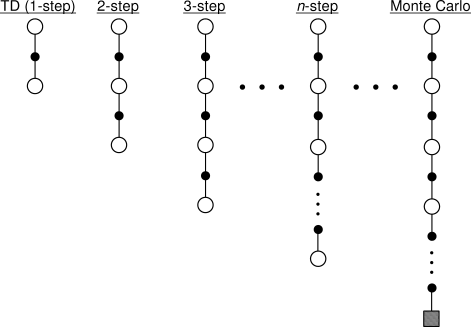
\includegraphics[width=\linewidth]{images/nStepTD.png}
\caption{Returns each based on a different amount of rewards and by using the state value as a proxy afterwards. This is not needed for Monte Carlo methods as they use all the future rewards. Source: \cite{Sutton1998ReinforcementIntroductionb}.}
\label{fig:nStepTD}
\end{figure}
The $n$-step target can be formulated as:
\begin{equation}
R_t^{(n)} = r_{t+1} + \gamma r_{t+2} + \dots + \gamma^{n-1}r_{t+n} + \gamma^n V_t(s_{t+n})
\end{equation}
There, we treat the terminal state as a state that always transitions to itself with zero reward. This way of treating an episodic task the same as a continuing task doesn't influence the result, even if we discount the returns. As such, all $n$-step returns that last up to or past termination have the same value as the complete return.\\
The increment to $V_t(s_t)$ is then defined by:
\begin{equation}
\Delta V_t(s_t) = \alpha \big[ R_t^{(n)} - V_t(s_t) \big]
\end{equation}
In on-line updating, the updates are done during the episode, as soon as a $\Delta V_t(s_t)$ is computed. In off-line updating, these increments are set aside and applied after the episode is done.\\
$n$-step TD methods are rarely used because they are inconvenient to implement. To compute $n$-step returns, you have to wait $n$ steps to observe the resultant rewards and states.\\

We can also take the weighted average of $n$-step return. This is called the forward view or theoretical view. The requirement is that the weights sum to 1. TD($\lambda$) is a particular way of doing this. The $\lambda$-return is defined by
\begin{equation}
R^\lambda_t = (1-\lambda) \sum_{n=1}^{\infty} \lambda^{n-1} R_t^{(n)}
\end{equation}
After a terminal state has been reached, all subsequent $n$-step returns are equal to $R_t$, so the $(1-\lambda)$ isn't applied. When $\lambda=1$, we will only have the conventional return $R_t$. The increment, $\Delta V_t(s_t)$, is:
\begin{equation}
\Delta V_t(s_t) = \alpha \big[ R_t^{\lambda} - V_t(s_t) \big]
\end{equation}
In this forward view, we look for each state visited forward in time to all the future rewards and decide how best to combine them. After looking forward from and updating one state, we move to the next and don't work with that state anymore. Future states, however, are viewed and processed repeatedly. This way of thinking is visualized in Figure \ref{fig:TDForwardView}.
\begin{figure}[H]
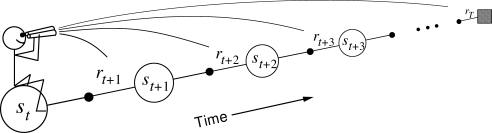
\includegraphics[width=\linewidth]{images/TDForwardView.png}
\caption{The forward view, where each state value is updated by looking forward to the states and their rewards that follow. Source: \cite{Sutton1998ReinforcementIntroductionb}.}
\label{fig:TDForwardView}
\end{figure}

The backward view can be seen as a practical version of the forward view, as it achieves the same but is easier to implement.
Here we have an additional memory variable associated with each state, the eligibility trace, denoted $e_t(s) \in \rm I\!R^+$. On each step, they are decayed by $\gamma \lambda$, and the eligibility trace for the one state visited on the step is incremented by 1. The increment $\Delta V_t(s_t)$ is then defined as such:
\begin{subequations}
\label{eq:backview}
\begin{align}
\delta_t &= r_{t+1} + \gamma V_t(s_{t+1}) - V_t(s_t) \label{eq:backview1} \\
\Delta V_t(s) &= \alpha \delta_t e_t(s), \qquad \text{for all} \quad s \in S \label{eq:backview2}
\end{align}
\end{subequations}
Here we work backwards and update backward to each prior state according to the state's eligibility trace at that time. This is visualized in Figure \ref{fig:TDBackwardView}.
\begin{figure}[H]
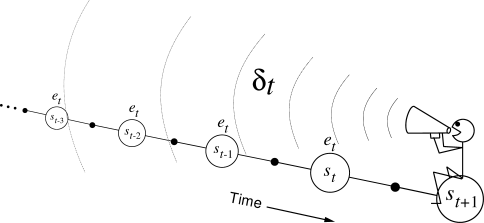
\includegraphics[width=\linewidth]{images/TDBackwardView.png}
\caption{The backward view, where the value of visited states are updated based on their eligibility values. Source: \cite{Sutton1998ReinforcementIntroductionb}.}
\label{fig:TDBackwardView}
\end{figure}
If we set $\lambda = 0$, then we only update the trace for $s_t$, thus getting TD(0). For larger values, with $\lambda < 1$, more of the preceding states are changed. The more distant states are changed by a smaller amount because the eligibility trace is smaller. This way, they are blamed less for the TD error.\\
If $\lambda = 1$ the credit given to earlier states falls only by $\gamma$ per step. If $\lambda = 1$ and $\gamma = 1$, then there is no decay at all and we achieve the Monte Carlo method for an undiscounted episodic task. This is known as TD(1). This TD(1) is more general however because it cannot only be applied to episodic tasks, but also to discounted continuing tasks. It can also be performed incrementally and on-line, while Monte Carlo methods have to wait until the episode is over. If the Monte Carlo control method does something bad, its behaviour cannot change during the same episode, while on-line TD(1) can (using $n$-step).\\
Both methods achieve the same weight update.\\

To combine TD($\lambda$) and Sarsa, called Sarsa($\lambda$), we need eligibility traces for each state-action pair: $e_t(s,a)$. As such, we do updates like this:
\begin{equation}
Q_{t+1}(s,a) = Q_t(s,a) + \alpha \delta_t e_t(s,a), \qquad \text{for all} \quad s,a
\end{equation}
where
\begin{equation}
\delta_t = r_{t+1} + \gamma Q_t(s_{t+1},a_{t+1}) - Q_t(s_t,a_t)
\end{equation}
and
\begin{equation}
e_t(s,a) = \begin{cases}
	\gamma \lambda e_{t-1}(s,a) + 1 & \text{if $s=s_t$ and $a=a_t$;} \\
	\gamma \lambda e_{t-1}(s,a) & \text{otherwise}.
\end{cases}
\qquad \text{for all $s,a$}
\end{equation}
This results in the following algorithm:\\
\begin{algorithm}[H]
\DontPrintSemicolon
Initialize $Q(s,a)$ arbitrarily\;
$e(s,a) \gets 0$ for all $s,a$\;
\For{each episode} {
	Initialize s,a\;
	\Repeat{$s$ is terminal} {
    	Take action $a$, observe reward $r$ and new state $s'$\;
        Choose action $a'$ from $s'$ with action selection policy using $Q$\;
        $\delta = r + \gamma Q(s',a') - Q_t(s,a)$\;
        $e(s,a) \gets e(s,a) + 1$\;
        \For{all $s,a$} {
        	$Q(s,a) \gets Q(s,a) + \alpha \delta e(s,a)$\;
            $e(s,a) \gets \gamma \lambda e(s,a)$\;
        }
        $s \gets s'$; $a \gets a'$\;
    }
}
\caption{Sarsa($\lambda$). Source: \cite{Sutton1998ReinforcementIntroduction}}
\end{algorithm}
Two methods exist to combine TD($\lambda$) and Q-learning and thus getting Q($\lambda$): There exists 2 different methods: Watkins' Q($\lambda$) and Peng's Q($\lambda$).\\
Here, we must cut off the look ahead until the first exploratory action instead of the episode's end. This is done because this exploratory action doesn't have any relationship with the greedy policy. Recall that Q-learning is an off-policy method and the policy learned about is not necessarily the same as the one used to select actions. As such, it can learn about the greedy policy while following a policy involving exploratory (suboptimal) actions.

For Watkins' Q($\lambda$), if $a_{t+n}$ is the first exploratory action, the longest backup is toward:
\begin{equation}
r_{t+1} + \gamma r_{t+2} + \dots + \gamma^{n-1} r_{t+n} + \gamma^n \max_a Q_t(s_{t+n},a)
\end{equation}
Where we assume off-line updating.\\
In the backward view, we update the eligibility traces just like in Sarsa, with the only exception that we don't use the eligibility trace of the previous time step when a suboptimal (exploratory) action is taken. We get the following result:
\begin{equation}
e_t(s,a) = I_{s s_t} * I_{a a_t} + \begin{cases}
	\gamma \lambda e_{t-1}(s,a) & \text{if $Q_{t-1}(s_t,a_t) = \max_a Q_{t-1}(s_t,a)$;} \\
    0 & \text{otherwise}
\end{cases}
\end{equation}
Where $I_{xy}$ is an identity indicator function, equal to $1$ if $x=y$ and $0$ otherwise. The Q update is defined by:
\begin{equation}
Q_{t+1}(s,a) = Q_t(s,a) + \alpha \delta_t e_t(s,a)
\end{equation}
Where
\begin{equation}
\delta_t = r_{t+1} + \gamma \max_{a'} Q_t(s_{t+1}, a') - Q_t(s_t,a_t)
\end{equation}
This results in the following pseudo-code:\\
\begin{algorithm}[H]
\DontPrintSemicolon
Initialize $Q(s,a)$ arbitrarily\;
$e(s,a) \gets 0$ for all $s,a$\;
\For{each episode} {
	Initialize s,a\;
	\Repeat{$s$ is terminal} {
    	Take action $a$, observe reward $r$ and new state $s'$\;
        Choose action $a'$ from $s'$ with action selection policy using $Q$\;
        $a^* \gets \argmax_b Q(s',b)$\;
        \If{$a^* = a'$} {
        	$a^* \gets a'$\;
        }
        $\delta = r + \gamma Q(s',a^*) - Q_t(s,a)$\;
        $e(s,a) \gets e(s,a) + 1$\;
        \For{all $s,a$} {
        	$Q(s,a) \gets Q(s,a) + \alpha \delta e(s,a)$\;
            \eIf{$a^* = a'$} {
            	$e(s,a) \gets \gamma \lambda e(s,a)$\;
            }{
            	$e(s,a) \gets 0$\;
            }
        }
        $s \gets s'$; $a \gets a'$\;
    }
}
\caption{Watkins' Q($\lambda$). Source: \cite{Sutton1998ReinforcementIntroduction}}
\end{algorithm}
Because exploratory actions happen often, backups won't be long and so eligibility traces won't have a lot of advantage anymore.\\
Peng's Q($\lambda$) tries to solve this, being a hybrid of Sarsa($\lambda$) and Watkin's Q($\lambda$). Its component backups are neither off- nor on-policy. The earlier transitions are each on-policy and the last transition uses the greedy policy. As such, all but the last uses the actual experiences. Because of this, for a fixed non-greedy policy, $Q_t$ converges to neither $Q^{\pi}$ nor $Q^{*}$, but some hybrid between the 2. If the policy is more greedy, the method may still converge to $Q^{*}$.\\

Replacing traces are a modified kind of eligibility traces that can yield a slightly better performance. With the traditional kind of traces (accumulating traces), the trace of a state is augmented by 1 when visiting it. With replacing traces, however, they are set to 1. Thus, we get the following update:
\begin{equation}
e_t(s) = \begin{cases}
\gamma \lambda e_{t-1}(s) & \text{if $s \neq s_t$;}\\
1 & \text{if $s=s_t$.}
\end{cases}
\end{equation}
Prediction or control algorithms using this are called replace-trace methods.
\begin{equation}
e_t(s,a) = \begin{cases}
1 + \gamma \lambda e_{t-1}(s,a) & \text{if $s=s_t$ and $a=a_t$;}\\
0 & \text{if $s=s_t$ and $a \neq a_t$;} \qquad \text{for all $s,a$}\\
\gamma \lambda e_{t-1}(s,a) & \text{if $s \neq s_t$.}
\end{cases}
\end{equation}

Another possible improvement if set correctly is a variable $\lambda$, which can be different at each time step $t$. It can for example depend on the current state: $\lambda_t = \lambda(s_t)$. It can be set to zero when we are sure about the estimate of the state $s_t$, so we don't have to use estimates of following states anymore. By setting it to $1$, we can achieve the opposite.

%Chapter 8
\subsection{Generalization and function approximation}
Normally, if there are a lot of possible states, it will take a long time to learn the estimates of all states. It is even possible that, after some time, previously unseen states will be encountered. This problem is possible when using continuous variables, images, \dots To solve this, we generalize states. As such, we can apply information of seen states to related states that haven't been visited yet. To do this, we combine standard reinforcement learning methods with generalization methods. A well known kind of generalization methods is called function approximation: it takes examples of a desired function and tries to approximate it. This is supervised learning (the input is the original value and the output to predict is the generalized value). The used supervised learning algorithm needs to be able to handle non-stationary target functions, as learning must be able to occur on-line. The error for the algorithm to minimize is the mean-squared error (MSE) between the true value of the state and the approximated one:
\begin{equation}
MSE(\overrightarrow{\theta_t}) = \sum_{s \in S} P(s) \big[ V^{\pi}(s) - V_t(s) \big]^2
\end{equation}
Where $\theta_t$ is a component of the model that the algorithm generated and $P$ is a distribution weighting the errors of different states. As there are less components $\overrightarrow{\theta_t}$ than states, the flexibility for approximation is limited. Because of this, we use $P$ to define the trade-offs of focusing on improving the approximation of some states at the expense of others. Usually, this distribution $P$ is the same as the one from which the states in the training examples are drawn from and thus the distribution of states at which backups are done. For minimizing the error over a certain distribution of states, it is of course preferred that the training examples come from the same distribution.\\
Another interesting distribution is the on-policy distribution, which describes the frequency with which states are encountered while the agent is interacting with the environment and selecting actions according to policy $\pi$. Minimizing the error over this distribution, we concentrate on states that actually occur while following the policy and ignoring others. Training examples for this distribution are also the easiest to get using Monte Carlo or TD methods because they generate backups from sample experience using the policy $\pi$.\\
%Minimizing the MSE may not lead to finding the best predictions. However, we have no alternative yet.\\
For simple function approximators such as linear ones, the best MSE we find might also be the global optimum. This is however rarely possible for more complex ones, e.g. kernel based methods or artificial neural networks, and they may stop at a local optimum. For many cases of interest in reinforcement learning, convergence to an optimum, i.e. achieving the highest possible reward, does not occur.\\

One of the most widely used function approximation methods is based on gradient descent. Here, the parameter vector is a column vector with a fixed number of real valued components, also called a weight vector: $\overrightarrow{\theta_t} = (\theta_t(1), \theta_t(2), \dots, \theta_t(n)^T$. $V_t(s)$ is a smooth differentiable function of $\overrightarrow{\theta_t}$ for all $s \in S$. At each time step $t$, we observe a new example $s_t \mapsto V^{\pi}(s_t)$. The order of the received states is not assumed to be the same as the order of gathering them from transitions in the environment. Even if we would give the exact $V^{\pi}(s_t)$, the function approximator has only limited resources and would not be able to approximate the function exactly. Thus, it must generalize.\\
Like already discussed, we assume that the states over which we want to minimize the MSE over come from the same distribution $P$ as the from examples.
%Found following definition on: https://en.wikipedia.org/wiki/Score_(statistics)
Gradient descent works by reducing the error by adjusting the parameters using the gradient, which is a vector of partial derivatives:
\begin{align}
\overrightarrow{\theta}_{t+1} &= \overrightarrow{\theta}_t - \frac{1}{2} \alpha \Delta_{\overrightarrow{\theta}_t} \big[ V^{\pi}(s_t) - V_t(s_t) \big]^2\\
&= \overrightarrow{\theta}_t + \alpha \big[ V^{\pi}(s_t) - V_t(s_t) \big] \Delta_{\overrightarrow{\theta}_t} V_t(s_t)
\end{align}
Where $\alpha$ is a positive step-size parameter and $\nabla_{\overrightarrow{\theta}_t}$ denotes the vector of partial derivatives for every function $f$. This vector is called the gradient of $f$ with respect to $\overrightarrow{\theta}_t$. The method is called gradient descent because the step with which we change $\overrightarrow{\theta}_t$ is proportional to the negative gradient of the MSE of the examples, i.e. in the direction of a lower MSE.\\
If $V^{\pi}(s_t)$ is unavailable because we only have a noise-corrupted version or one with backed-up values, we can simple use $v_t$ instead of $V^{\pi}(s_t)$:
\begin{equation}
\overrightarrow{\theta}_{t+1} = \overrightarrow{\theta}_t + \alpha \big[ v_t - V_t(s_t) \big] \Delta_{\overrightarrow{\theta}_t} V_t(s_t)
\end{equation}
If $v_t$ is an unbiased estimate and so $E\{v_t\} = V^{\pi}(s_t)$ for each $t$, then $\overrightarrow{\theta}_t$ is guaranteed to converge to a local optimum under stochastic approximation conditions for decreasing the step-size parameter $\alpha$. This is the case for Monte Carlo state-value prediction.\\

An important special case is when the approximate function $V_t$ is a linear function of the parameter vector, $\overrightarrow{\theta}_t$. For every state $s$, there is a column vector of features $\overrightarrow{\phi}_s = (\phi_s(1), \phi_s(2), \dots, \phi_s(n))^T$, with the same number of components as $\overrightarrow{\theta}_t$. The approximate state-value function is then given by:
\begin{equation}
V_t(s) = \overrightarrow{\theta}_t^T \overrightarrow{\phi}_s = \sum_{i=1}^n \theta_t(i) \phi_s(i)
\end{equation}
The gradient with respect to $\overrightarrow{\theta}_t$ is then:
\begin{equation}
\nabla_{\overrightarrow{\theta}_t} V_t(s) = \overrightarrow{\phi}_s
\end{equation}
As can be seen, this update is rather simple. Furthermore, there is only one optimum (or several ones which are equally good), $\overrightarrow{\theta}^{*}$. As a result, the method is guaranteed to converge to or near a local optimum.\\
Note that this linear form doesn't allow for the representation of interactions between features, for example when the presence of a certain features is good only if another feature is absent. For this, we need to introduce features that are combinations of feature values.\\

\subsubsection{Coarse coding}
Coarse coding is the representation of a state with features that overlap, for example a binary feature that is $1$ when the coordinate given by a $x$ and $y$ feature lies in a circle. If 2 points \textit{A} and \textit{B} have circles "in common", there will be some generalization between them, as the features for both points for those circles will be 1. This is shown in Figure~\ref{fig:coarsecoding1}. The more features in common, the greater this effect.
\begin{figure}[H]
\captionsetup{width=0.8\textwidth}
\centering
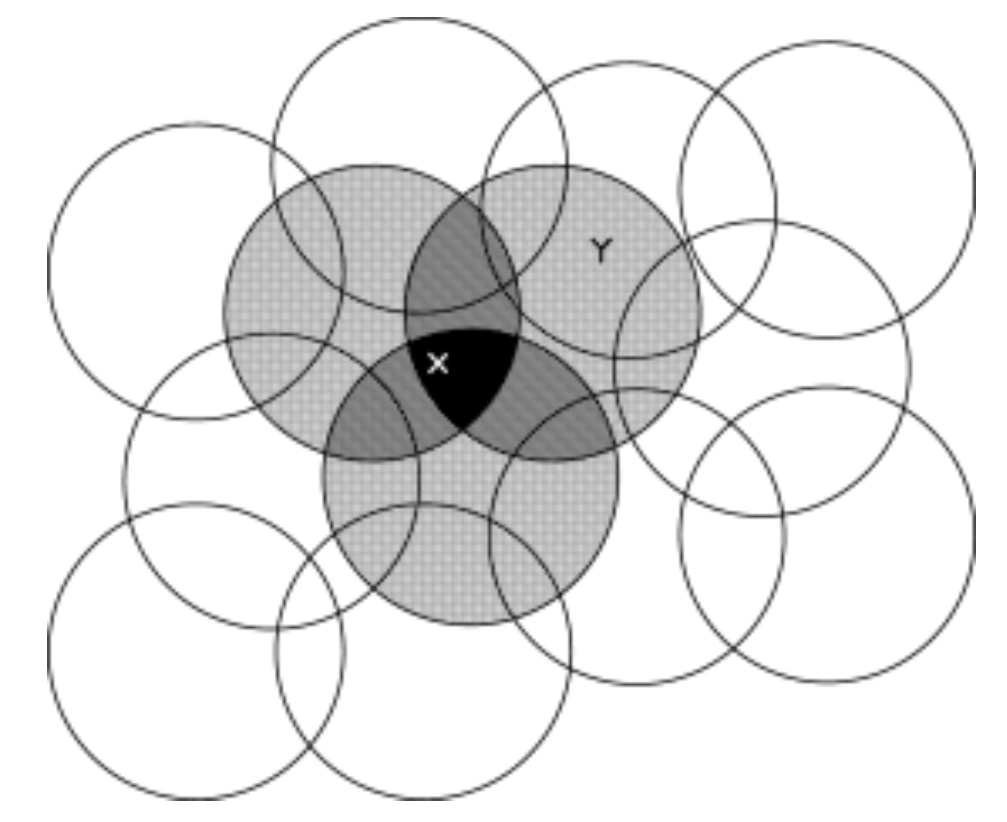
\includegraphics[width=0.5\linewidth]{images/coarsecoding1.png}
\caption{$X$ and $Y$ share 1 feature, as both points lie in the same receptive field, a circle. Thus, slight generalization from $X$ to $Y$ is possible. Source: \cite{Sutton1998ReinforcementIntroductionb}.}
\label{fig:coarsecoding1}
\end{figure}
If the circles are small or large, generalization will be over respectively a short or large distance. The nature of the generalization is also affected by the shape of the features' receptive fields.  This can be seen in Figure~\ref{fig:coarsecoding2}. The fineness of discrimination is however only determined by the total number of features.
\begin{figure}[H]
\captionsetup{width=0.8\textwidth}
\centering
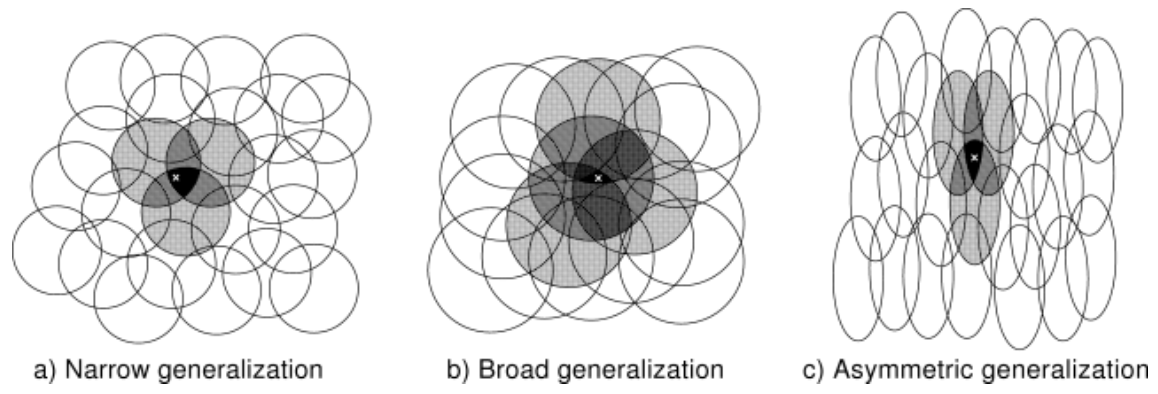
\includegraphics[width=0.8\linewidth]{images/coarsecoding2.png}
\caption{Generalization depends on the shape of the receptive fields of the features. When multiple features' receptive fields overlap, the generalization is broad and narrow when only few of them overlap. Source: \cite{Sutton1998ReinforcementIntroductionb}.}
\label{fig:coarsecoding2}
\end{figure}

In tile encoding, a form of coarse encoding, the fields of the features are grouped into exhaustive partitions of the input space, called tilings. These tilings are defined by ranges of values for state attributes that they cover. For one specific tiling, the state can only lie in the ranges of 1 tile. As such, maximally one feature is active in each tiling and the total number of features present is always the same as the number of tilings. This allows us to set the step-size parameter $\alpha$ (used in formula \ref{eq:backview1}) in an easy, intuitive way. We can for example choose $\alpha = \frac{1}{m}$, where $m$ is the number of tilings. This results in exact one-trial learning. When the example $s_t \mapsto v_t$ is received, then the new value will be $V_{t+1}(s_t) = v_t$, whatever the prior value $V_t(s_t)$ was. For a slower change using for example $\alpha=\frac{1}{10m}$, one would move one-tenth of the way to the target in one update.\\
The weighted sum to make up the approximate value function is almost trivial to compute, as in tile coding only binary features are used. Instead of performing $n$ multiplications and additions, we compute the indices of the $m<<n$ present features and then add up the $m$ corresponding components of the parameter vector. The eligibility trace computation is also easier because the components of the gradient $\nabla_{\overrightarrow{\theta}} V_t(s_t)$ are either $0$ or $1$.\\
An easy to compute form of tilings are grid-like ones. Different tilings may also be used, ideally offset by different amounts. The width and shapes should match the width of generalization that is expected to be optimal. The denser the tiling, the more fine-grained the desired function can be, but also the greater the computational cost of updating. The width or shape of each tile must not be uniform or regular-shaped (like a square) however. One can also use stripes, diamond shapes, \dots To reduce memory requirements, hashing can be used. A large tiling can be collapsed in such way into a much smaller set of tiles. This hashing produces tiles consisting of non-contiguous, disjoint regions randomly spread throughout the state space, but that still form an exhaustive tiling.\\
Radial basis functions are a generalization of coarse coding that allows for continuous-valued features: in the interval $[0,1]$ instead of just $0$ or $1$. This way, we can reflect various degrees to which the feature is present. A typical RBF feature, $i$, has a Gaussian (bell-shaped) response $\phi_s(i)$ dependent only on the distance between the state and the feature's centre state, $c_i$ and relative to the feature's width $\sigma_i$:
\begin{equation}
\phi_s(i) = e^{-\frac{||s-c_i||^2}{2 \sigma^2_i}}
\end{equation}
The advantage of this method is that they produce approximate functions that vary smoothly and are differentiable. The disadvantage is that $\sigma_i$ and $c_i$ must be tuned manually and that non-linear RBF networks are computationally complex.\\

%Kanerva coding
\subsubsection{Kanerva coding}
When the states have a high number of attributes, the previous methods can become impractical because of their computational complexity, even if we apply hashing. In the worst case, the complexity of the target function scales with the size of the state space. However, it is possible that some attributes are not useful for the learning algorithm and it would we better if those do not contribute to the complexity. This way, adding dimensions may not lead to an exponential increase in computational complexity.\\
A way of achieving this is called Kanerva coding, where we choose binary features that correspond to particular prototype states. These are randomly selected from the entire state space. The receptive field of such a feature is all states that are sufficiently close to the prototype. This means that there is a feature for every prototype state and it is set to 1 if the state is close to that prototype state and 0 otherwise. The chosen distance is the hamming distance for a binary state space (e.g. in case of a bitwise representation of states), which is the number of bits at which two states differ.
Using Kanerva coding, the complexity of the functions depends entirely on the number of used features, i.e. the number of prototype states, instead of the dimensionality. The amount of prototypes can be tuned such that the computational complexity and/or the performance improves.\\

\subsubsection{Function approximation for control}
To use function approximation for control, we use the action-value function $Q_t \approx Q^{\pi}$, that is represented as a parametrised functional form with parameter vector $\overrightarrow{\theta}_t$. Instead of only using training examples with $s_t$, they are now of the form $s_t, a_t \mapsto v_t$. The target output $v_t$ can be any approximation of $Q^{\pi}(s_t,a_t)$, including the usual backed-up values such as the full Monte Carlo return $R_t$ or the one-step Sarsa return $r_{t+1} + \gamma Q_t(s_{t+1}, a_{t+1})$. The gradient-descent update is now:
\begin{equation}
\overrightarrow{\theta}_{t+1} = \overrightarrow{\theta}_t + \alpha \big[ v_t - Q_t(s_t,a_t) \big] \nabla_{\overrightarrow{\theta}_t} Q_t(s_t,a_t)
\end{equation}
To select an action, we can just use a greedy (in off-policy methods) or $\epsilon$-greedy (in on-policy methods) approach.\\
To use traces along with function approximation methods, we cannot set the trace of a state, because there are only traces for components of $\overrightarrow{\theta}_t$. Instead, we set the trace for each feature $i$ that the the current encountered state has.\\
We can also set the traces of all non-selected actions to zero in the states encountered. To do this, for each state encountered, we first clear the traces of all features for the state and the actions not selected and then we set to 1 the traces of the features for the state and the action that was selected.\\

%Off-policy bootstrapping
\subsubsection{Bootstrapping}
Bootstrapping is the updating of a value estimate based on other value estimates. This is done by TD and DP methods, but not by Monte Carlo methods. TD($\lambda$) is a bootstrapping method when $\lambda <1$, but not when $\lambda = 1$. Although the latter involves bootstrapping within an episode, afterwards the effect over a complete episode is the same as the non-bootstrapping Monte Carlo update. Bootstrapping methods such as TD($\lambda$) are harder to combine with function approximation because they only find near-minimal MSE solutions (only for the on-policy distribution) instead of the minimal MSE using for example linear, gradient-descent function approximation for any distribution of training examples, $P$.\\
The restriction of convergence is especially a problem for off-policy methods such as Q-learning and DP methods because they do not backup states (or state-action pairs) with exactly the same distribution as the distribution of states we encounter when following the policy of which we want to estimate the value function. Off-policy bootstrapping combined with function approximation can even lead to divergence and infinite MSE.\\

Bootstrapping looks like a bad idea because non-bootstrapping methods are more easy and reliably used with function approximation and can be applied over a broader range of conditions. Non-bootstrapping methods also achieve a lower error in approaching the value function, even when backups are done according to the on-policy distribution \citep{ML}. In practice, however, bootstrapping methods achieve better performance. When $\lambda$ approaches $1$, which is the non-bootstrapping case, the performance becomes much worse.

%Chapter 9
\subsection{Planning and Learning}
A model is something that can be used by an agent to predict the resulting state and reward of doing an action in the environment. Distribution models give a probability for each possibility, whereas sample models just return one of the possibilities. The model can be used to simulate experiences because as it can be used to simulate several transitions and as such to simulate entire episodes.\\
Planning is the computational process of using this model and producing/improving a policy. State-space planning means the search through the state space for an optimal policy or path to a goal. In plan-space planning, we search through the space of plans. This includes evolutionary methods and partial-order planning. In the latter, the ordering of the steps is not fully defined in all the stages of planning.
\begin{figure}[H]
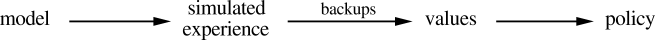
\includegraphics[width=\linewidth]{images/modelplanning.png}
\label{fig:modelplanning}
\end{figure}
Planning uses simulated experience, whereas learning uses real experience. Learning algorithms that only require experience as input can be used with real experience as well as simulated experience.\\

We planning is done online, new information gained from the interaction may change the model and influence planning. If decision-making and model-learning are both computationally expensive, the resources assigned to them must be divided.\\
Real experience can be used by a planning agent in two ways: for improving the model (such that it more accurately represents the real environment), named \textit{model-learning}, and for directly improving the value function and as such the policy, called \textit{direct reinforcement learning}. Because the model is used by planning methods to influence the policy, it can be called \textit{indirect reinforcement learning}. Indirect models are complex but are able to achieve a better performance with less amount of experience. Direct methods are simpler and are not affected by biases that are present in the models used by indirect methods.\\
Dyna-Q is an algorithm that combines planning, acting, model-learning and direct-RL. The planning method is a random-sample on-step tabular Q-planning method. The direct RL method is one-step tabular Q-learning. The model-learning method is also table-based and assumes the world is deterministic. This means that it doesn't use probabilities and just returns the previously experienced state and reward that was received after the queried state-action pair. The Q-planning algorithm only samples randomly from state-action pairs that have already been experienced, so the model is never queried with unknown pairs. Typically, as in Dyna-Q, the same reinforcement learning method is used both for learning from real experience and for planning from simulated experience.

Without planning, each episode adds only one additional step to the policy. With planning, also only one step is added during the first episode, but during the second one, an extensive planning policy can be applied that reaches back almost to the start state. The result of this is shown in Figure \ref{fig:withwithoutplanning}.
\begin{figure}[H]
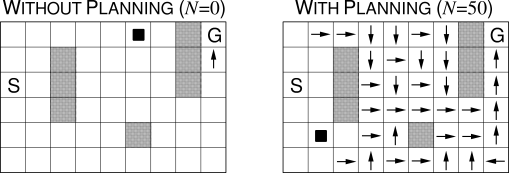
\includegraphics[width=\linewidth]{images/withwithoutplanning.png}
\caption{Difference in computed optimal actions when using no planning method and when using one. Source: \cite{Sutton1998ReinforcementIntroductionb}.}
\label{fig:withwithoutplanning}
\end{figure}

It can be seen that models may be able to fill in correct information. However, this is not always the case. Models may be wrong because only a limited number of samples have been observed, because of an imperfect function approximation that generalized wrongly or because the environment has changed and this hasn't been observed yet. When using this incorrect model, a sub-optimal policy will be computed. When the model is too optimistic, the algorithm will try to exploit this and notice that the optimistic values do not exist and will correct them. This optimism is for example discovered when a way in a maze gets blocked suddenly.\\
There is a larger problem when the environment changes such that there are better opportunities than there were before. This "modelling error" may not be detected for a long time. In a maze, this may mean that suddenly a shorter path becomes available but the Dyna-Q algorithm doesn't detect it for a long time (or not at all) and keeps choosing the sub-optimal path.\\
The general problem here is the trade-off between exploitation and exploration. As the algorithms did not try actions that were computed as being sub-optimal in the policy, the new, optimal path was never discovered. We would like to explore changes in the environment, but without degrading too much the performance.\\
The Dyna-Q+ algorithm is a heuristic algorithm that tries to find a good balance and achieve and practical solution. It encourages using actions that haven't been tried for a long time in the current state. It does so by increasing the reward of that transition by a value relative the the number of steps since the last use of the action. This way, exploration is encouraged because now taking that action seems better.\\

The previous Dyna agents simulated transitions starting from state-action pairs that were selected uniformly at random. However, focusing on certain state-action pairs may be more useful than others. In the start, for example, most state-action pairs still have a value of zero. As such, their is no use in simulating these transitions. Only transitions into states prior to the goal or from the state to the goal are useful to simulate. Later on, there are more and more useful backups. However, this may again result in sampling from too many backups. It may be more useful to focus on transitions that would do the most good.\\
When a value of a state has changed, the only useful transitions are those to this changed state. Afterwards, the transitions leading to these can be simulated as well, and so on. This way, we work backwards from the changed state.\\
Again, we will have a lot of state-action pairs that can be backed up. Still, not all of them may be equally useful. The values of some states may have changed a lot, and as such the predecessor pairs of those are more likely to change a lot. To use this information, we insert backups of predecessors of changed states into a priority queue, sorted by the size of the change. We only insert it if the priority is larger than some threshold.\\
The mentioned algorithms have the problem of relying on the fact that states are discrete. When function approximation is used (because the states are continuous), a single backup could influence a lot of other states. It is not clear if these states could be identified or processed efficiently.\\
When using stochastic environments, the only difference is that we need to do a full backup and take into account all the possible next states along with their possibilities, instead of doing a sample backup.\\

The computation of (one-step) backups can differ in 3 possible ways: The first is the binary difference of whether they backup state values or action values. The second one is whether they estimate the value for the optimal policy or for an arbitrary given policy. The last one is whether the backups are full backups or just sample backups. This results in 8 cases, of which 7 result in useful kind of backups. These are shown in Figure \ref{fig:backuptypes}.
\begin{figure}[H]
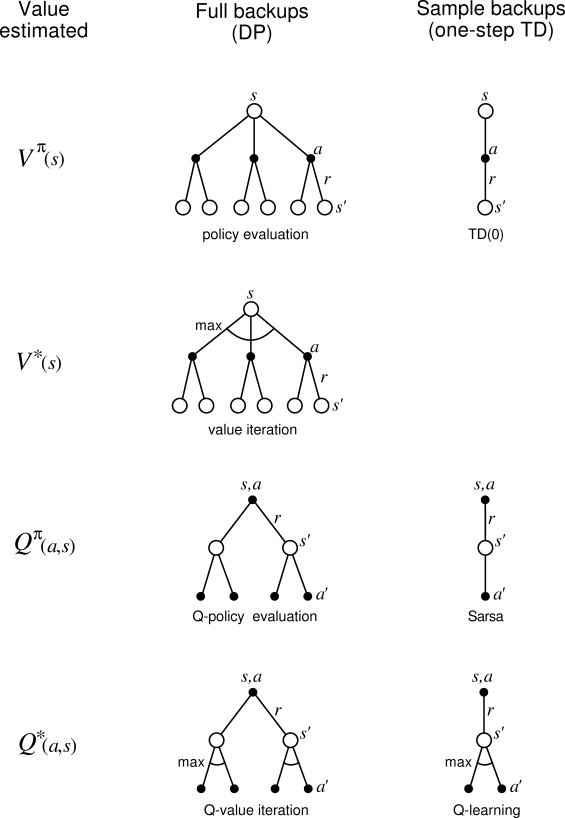
\includegraphics[width=\linewidth]{images/backuptypes.png}
\caption{Different kind of backups, depending on what value they backup and whether they do full backups or sample backups. Source: \cite{Sutton1998ReinforcementIntroductionb}.}
\label{fig:backuptypes}
\end{figure}
Full backups are only possible when we know the transition distribution ($\mathcal{P}^a_{ss'}$) and reward distribution ($\mathcal{R}^a_{ss'}$). Otherwise, we have to do sample backups using sample transitions from the environment or from a sample model. Full backups may give a better estimate because they are uncorrupted by the sample error, but they also require more computation because they need to do a lot more backups: they consider all the possible next states ($b$, the branching factor) instead of just one next state. This is probably not feasible to use with planning when there is not a lot of time available.\\

In dynamic programming, we perform sweeps through the entire state(-action) space. As we already said, this may take a lot of time. In many tasks, some states may be irrelevant as they are only visited with a low probability and/or using very poor policies. The second possibility is to sample from the state(-action) space according to a distribution. If we would sample uniformly, we would have the same problems as the already explained exhaustive sweep.\\
We could also use the distribution observed when following the current policy. This is easily generated by just starting in the begin state and simulating until the terminal state (in case of an episodic task, otherwise it just keeps simulating). Here we simulate explicit individual trajectories and we perform backups using the state or state-action pairs encountered. This way of generating experience is called \textit{trajectory sampling}.\\
If we would have an explicit representation of the on-policy distribution, we could sweep through all states, weighting the backup according to this distribution. This however will gives us again a large computational cost. We could also sample and update individual state-action pairs from this distribution, but this would not give a huge benefit over simulating the trajectories. Moreover, computing the on-policy distribution may require itself a big computational cost, as the distribution changes whenever the policy changes.\\
Focusing on the on-policy distribution may be good because uninteresting parts of the state(-action) space may be ignored. However, it may also result in backing op the same part of the space over and over again.

In experiments it was seen that sampling according to the on-policy distribution results in faster planning initially and retarded planning in the long run than when using the uniform distribution \citep{ML}. The effect is stronger with smaller branching factors, as well as when the number of states increased. In the short term, using the on-policy distribution results in performing backups on states that are near descendants of the start state. In the long run, this distribution may be bad for us because we keep focusing on the same states, which already have more or less their correct values. Other states may be more interesting to explore, which is why the exhaustive unfocused approached may be better in this case, at least for small problems (because of the computational cost).\\

The idea of heuristic search is to make improved action selections given a value function. As such, it is a part of the policy computation. For a state, it considers a tree of all possible continuations. The approximate value function is applied to the leaf nodes and then backed up (max-backups like for $V^{*}$ and $Q^{*}$) towards the current state at the root. Once these backed-up values are computed, we can choose the best of them and discard the rest. ($\epsilon$-)greedy action selection methods are alike, as they only compute the backup values for all the possible next states (not for the states after those).\\
By searching deeper, we obtain better action selections. This can eliminate the problem of imperfect action selection and the actions will be near optimal. However, more computation time is needed for deeper searches.\\
Besides using it for action selection, heuristic search can also suggest ways to distribute the backups such that the optimal value function is approximated faster and to make the search more efficient. Ideally, the tree should be grown and explored deeper for actions that seem most likely to be best. Practically, this could be done by updating state-action pairs of which the value is close to the maximum available from the state.\\
Much of the effectiveness of heuristic search is due to its search tree being tightly focused on the states and actions that might immediately follow the current state. In a state, you select the actions of which the state-action value urgently needs to be accurate. Besides this, the required memory resources is limited. This 2 ways of focusing may be the reasons why heuristic search is effective.

\subsection{Policy gradient}
%By David Silver.\\

Here, we parametrise the policy instead of the state value or state-action value function.
Methods that parametrise the policy tend to have better convergence properties \citep{Sutton1999PolicyApproximation}.
No value must be stored for every specific state and action. This is useful in problems where the state and/or action space is high-dimensional and/or continuous. Last, they can also learn policies where a probability is provided for every action.
However, policy gradient methods also come with a few disadvantages. They typically converge to a local optimum instead of a global optimum. It is also rather hard to evaluate a policy and it can have a high variance.\\
The policy gradient has the form of $\pi_{\theta}(s,a)$. The way of measuring the quality of a policy (i.e. how well it performs in an environment) depends on the type of environment:
\begin{itemize}
\item Episodic environments: use the value of the start state: $J_1(\theta) = V^{\pi_{\theta}}(s_1) = E_{\pi_{\theta}} [v_1]$
\item Continuing environments: use the average value: $J_{avV}(\theta) = \sum_s d^{\pi_{\theta}}(s)V^{\pi_{\theta}}(s)$
\item or the average reward per time step: $J_{avR}(\theta) = \sum_s d^{\pi_{\theta}} \sum_a \pi_{\theta}(s,a) R_s^a$
\end{itemize}
Where $d^{\pi_{\theta}}$ is the stationary distribution of the Markov chain for $\pi_{\theta}$. The stationary distribution $\bar{\pi}$ of a Markov distribution $P$ is a probability distribution such that $\bar{\pi} = \bar{\pi} P$. It can be thought of as denoting how much time is spent in each state. This way, values/rewards of states which are visited often are given a higher importance.\\
As such, we need to find the parameters $\theta$ that maximize $J(\theta)$. This optimization problem can be solved using approaches that don't use a gradient, such as hill climbing or genetic algorithms. However, here we focus on gradient descent. In this case, we move the parameter values along the gradient using the quality function: $\Delta \theta = \alpha \nabla_{\theta} J(\theta)$, where $\alpha$ is the step-size parameter and $\nabla_{\theta} J(\theta)$ is the partial derivative for every dimension of $\theta$. To estimate each partial derivative, we can compute the policy objective function $J(\theta)$ for a slightly changed value of $\theta$, determined by $\epsilon$. For each dimension $k$, this is:
\begin{equation}
\frac{\partial J(\theta)}{\partial \theta_k} \approx \frac{J(\theta + \epsilon u_k) - J(\theta)}{\epsilon}
\end{equation}
where $u_k$ is a one-hot vector with a value of $1$ in dimension $k$ and $0$ elsewhere. This kind of gradient is called a Finite Difference gradient. It is a simple, black-box way that works for every policy (because we don't need the derivative), but it is inaccurate and inefficient. We also need to determine the value of $\epsilon$ ourselves, which influences the accuracy.\\

Instead, we will solve the problem analytically. We assume that the policy is differentiable when it is non-zero and that we know the gradient.

%What is likelihood?
% Likelihood is a funny concept. It’s not a probability, but it is proportional to a probability. The likelihood of a hypothesis (H) given some data (D) is proportional to the probability of obtaining D given that H is true, multiplied by an arbitrary positive constant (K). In other words, L(H|D) = K · P(D|H). Since a likelihood isn’t actually a probability it doesn’t obey various rules of probability. For example, likelihood need not sum to 1.

% A critical difference between probability and likelihood is in the interpretation of what is fixed and what can vary. In the case of a conditional probability, P(D|H), the hypothesis is fixed and the data are free to vary. Likelihood, however, is the opposite. The likelihood of a hypothesis, L(H|D), conditions on the data as if they are fixed while allowing the hypotheses to vary.

% The distinction is subtle, so I’ll say it again. For conditional probability, the hypothesis is treated as a given and the data are free to vary. For likelihood, the data are a given and the hypotheses vary.
% Source (with more explanation): https://alexanderetz.com/2015/04/15/understanding-bayes-a-look-at-the-likelihood/
\todo{Explain likelihood?}
Likelihood ratios use the following identity:
\begin{align}
\nabla_{\theta}\pi_{\theta}(s,a) &= \pi_{\theta}(s,a) \frac{\nabla_{\theta}\pi_{\theta}(s,a)}{\pi_{\theta}(s,a)}\\
&= \pi_{\theta}(s,a) \nabla_{\theta} \log \pi_{\theta}(s,a)
\end{align}
Writing it using the $\log$ is possible because $(\log f)' = \frac{f'}{f}$. The score function is $\nabla_{\theta} \log \pi_{\theta}(s,a)$.\\
This can now be used with for example a softmax policy. Here, we weight actions using a linear combination of features: $\phi(s_a)^T \theta$. The probability of an action is then the following proportion:
\begin{equation}
\pi_{\theta}(s,a) \propto \rm{e}^{\phi(s,a)^T \theta}
\end{equation}
The score function is here defined as being:
\begin{equation}
\nabla_{\theta} \log \pi_{\theta}(s,a) = \phi(s,a) - E_{\pi_{\theta}}[\phi(s,\cdot)]
\end{equation}
When having a continuous action space, it is better to use a Gaussian policy, where the mean is a linear combination $\mu(s) = \phi(s)^T \theta$ and the variance can be either fixed or also parametrised. The policy is then $a \sim N(\mu(s), \sigma^2)$. The score function here is defined as being:
\begin{equation}
\nabla_{\theta} \log \pi_{\theta}(s,a) = \frac{(a-\mu(s))\phi(s)}{\sigma^2}
\end{equation}
We can now use the likelihood ratios to compute the policy gradients for one-step Markov decision processes:
\begin{align}
J(\theta) &= E_{\pi_{\theta}}[r]\\
&= \sum_{s \in S} d(s) \sum_{a \in A} \pi_{\theta}(s,a) R(s,a)\\
\nabla_{\theta} J(\theta) &= \sum_{s \in S} d(s) \sum_{a \in A} \pi_{\theta}(s,a) \nabla_{\theta} \log \pi_{\theta}(s,a) R(s,a)\\
&= E_{\pi_{\theta}} [\nabla_{\theta} \log \pi_{\theta}(s,a)r]
\end{align}
%Got it from here: https://pdfs.semanticscholar.org/eb5b/459c8a3e56064158fb3514eeab763486e437.pdf but I interpreted it wrong. However, REINFORCE may do something like , by averaging these gradients over multiple trajectories. So it may be useful to look into it
% \todo{Next part is wrong, see comment}
% When considering multiple trajectories $\tau \sim p_\theta(\tau) = p(\tau \vert \theta)$, we can compute the quality like this:
% \begin{equation}
% J(\theta) = \int_{T} p_{\theta}(\tau \vert \pi)r(\tau) d\tau
% \end{equation}
% Where $r(\tau) = \sum_{k=0} \gamma^k r_k$. We again have a gradient:
% \begin{equation}
% \nabla_{\theta}J_{\theta} = \nabla_{\theta} \int_{T} p_{\theta}(\tau \vert \pi)r(\tau) d\tau = \int_T \nabla_{\theta} p_{\theta}(\tau \vert \pi) r(\tau) d\tau
% \end{equation}
% Using again the $\log$ trick, we get:
% \begin{align}
% \nabla_{\theta}J(\theta) &= \int_T p_{\theta}(\tau \vert \pi) \nabla \log p_{\theta} (\tau \vert \pi) r(\tau) d\tau\\
% &= E[\nabla_{\theta} \log p_{\theta}(\tau \vert \pi)r(\tau)]\\
% &\approx \frac{1}{K} \sum_{k=1}^K \nabla_{\theta} \log p_{\theta}(\tau \vert \pi) r(\tau_k)
% \end{align}
The Policy Gradient theorem states that we can use this for multi-step MDP's \citep{Sutton1999PolicyApproximation}. We can do this by replacing the reward with the state-action value:
\begin{equation}
E_{\pi_{\theta}} [\nabla_{\theta} \log \pi_{\theta}(s,a)Q^{\pi_{\theta}}(s,a)]
\end{equation}
Monte-Carlo policy gradients use this policy gradient theorem and update parameters using stochastic gradient descent. For this, a return $v_t$ is used as an unbiased sample of $Q^{\pi_{\theta}}(s,a)$. The resulting algorithm is called \texttt{REINFORCE}:\\
\begin{algorithm}[H]
\DontPrintSemicolon
Initialize $\theta$ arbitrarily\;
\For{each episode $\{s_1, a_1, r_2, \dots, s_{T_1}, a_{T_1}, r_T\} \sim \pi_{\theta}$} {
	\For{$t=1$ to $T-1$} {
    	$\theta \gets \theta + \alpha \nabla_{\theta} \log \pi_{\theta}(s_t,a_t)v_t$
    }
}
\Return $\theta$
\caption{REINFORCE}
\end{algorithm}

The problem with the Monte-Carlo policy gradient is that it has a high variance. This can be solved by using an actor-critic method. The critic is used to update the state-action value function parameters $w$, such that $Q_w(s,a) \approx Q^{\pi_{\theta}}(s,a)$, while the actor updates the policy parameters $\theta$ in the direction suggested by the critic. These actor-critic algorithms follow an approximate policy gradient:
\begin{align}
\nabla_{\theta}J(\theta) &\approx E_{\pi_{\theta}}[\nabla_{\theta} \log \pi_{\theta}(s,a) Q_w(s,a)]\\
\Delta \theta &= \alpha \nabla_{\theta} \log \pi_{\theta}(s,a) Q_w(s,a)
\end{align}
The critic function can be seen of a way of evaluating how good the policy is for the current $\theta$. A simple way of computing $Q_w(s,a)$ is simply a linear function of $w$ and $\phi(s,a)$: $Q_w(s,a) = \phi(s,a)^T w$. The algorithm, named \texttt{QAC} then is:\\
\begin{algorithm}[H]
\DontPrintSemicolon
Initialize $s,\theta$\;
Sample $a \sim \pi_{\theta}$\;
\For{each step} {
	Sample reward $r = R_s^a$; sample transition $s' \sim P_s^a$\;
    Sample action $a' \sim \pi_{\theta}(s',a')$\;
    $\delta = r + \gamma Q_w(s',a') - Q_w(s,a)$\;
    $\theta = \theta + \alpha \nabla_{\theta} \log \pi_{\theta}(s,a)Q_w(s,a)$\;
    $w \gets w + \beta \delta \phi (s,a)$\;
    $a \gets a'$, $s \gets s'$\;
    }
\caption{QAC}
\end{algorithm}
For a function approximation to be compatible, it needs to fulfil 2 conditions:
\begin{itemize}
\item The value function approximator is compatible to the policy: $\nabla_w Q_w(s,a) = \nabla_{\theta} \log \pi_{\theta}(s,a)$
\item The value function parameters w minimize the mean-squared error: $\epsilon = E_{\pi_{\theta}} [(Q^{\pi_{\theta}}(s,a) - Q_w(s,a))^2]$
\end{itemize}
The policy gradient will then be exactly:
\begin{equation}
\nabla_{\theta}J(\theta) = E_{\pi_{\theta}} [\nabla_{\theta} \log \pi_{\theta}(s,a) Q_w(s,a)]
\end{equation}
To reduce the variance in the policy gradient we subtract the baseline function $B(s)$ from it. This doesn't change the expectation:
\begin{align}
E_{\pi_{\theta}} [\nabla_{\theta} \log \pi_{\theta}(s,a)B(s)] &= \sum_{s \in S} d^{\pi_{\theta}}(s) \sum_a \nabla_{\theta} \pi_{\theta}(s,a)B(s)\\
&= \sum_{s \in S} d^{\pi_{\theta}}B(s)\nabla_{\theta} \sum_{a \in A} \pi_{\theta} (s,a)\\
&= 0
\end{align}
A good baseline function is the state value function: $B(s) = V^{\pi_{\theta}}$. When this is used as a baseline function, we can rewrite the policy gradient using the advantage function $A^{\pi_{\theta}}(s,a)$:
\begin{align}
A^{\pi_{\theta}}(s,a) &= Q^{\pi_{\theta}}(s,a) - V^{\pi_{\theta}}(s)\\
\nabla_{\theta}J(\theta) &= E_{\pi_{\theta}}[\nabla_{\theta} \log \pi_{\theta}(s,a) A^{\pi_{\theta}}(s,a)]
\end{align}
This still reduces the variance. The critic should now estimate the advantage function. This can be done by estimating both $V^{\pi_{\theta}}(s)$ and $Q^{\pi_{\theta}}(s,a)$. With those 2 function approximators we then get:
\begin{align}
V_v(s) &\approx V^{\pi_{\theta}}(s)\\
Q_w(s,a) &\approx Q^{\pi_{\theta}}(s,a)\\
A(s,a) &= Q_w(s,a) - V_v(s)
\end{align}
For updating those values, we can again use temporal difference learning. The TD error is:
\begin{equation}
\delta^{\pi_{\theta}} = r + \gamma V^{\pi_{\theta}}(s') - V^{\pi_{\theta}}(s)
\end{equation}
This is an unbiased estimate of the advantage function:
\begin{align}
E_{\pi_{\theta}}[\delta^{\pi_{\theta}} | s,a] &= E_{\pi_{\theta}}[r + \gamma V^{\pi_{\theta}}(s') | s,a] - V^{\pi_{\theta}}(s)\\
&= Q^{\pi_{\theta}}(s,a) - V^{\pi_{\theta}}(s)\\
&= A^{\pi_{\theta}}(s,a)
\end{align}
As such, we can use this TD error to compute the policy gradient:
\begin{equation}
\nabla_{\theta}J(\theta) = E_{\pi_{\theta}}[\nabla_{\theta} \log \pi_{\theta}(s,a) \delta^{\pi_{\theta}}]
\end{equation}
In practice, we use the function approximator of the critic function for the value function, using the critic parameters $v$:
\begin{equation}
\delta_v = r + \gamma V_v(s') - V_v(s)
\end{equation}

\section{Deep learning}
%Review by \cite{LeCun2015DeepLearning}.\\

Before deep learning, raw data had to be transformed into an internal representation using manually crafted features usable for learners. In deep learning, these features are learned by itself, as it is a representation-learning method. Furthermore, different levels of representation can be used. Each level builds upon the previous one, starting from the input itself, and represents it in a more abstract way. These abstractions are generated as to recognize aspects of the input that are important for the task. Because of this, it is possible that small variations in the input have no influence on the abstraction and output. Because these abstractions are learned automatically, there is no need anymore to create internal representations manually, which require more work as it is different for every kind of task. The generated abstractions may also recognize useful patterns in the data that might not be represented using the hand-crafted features.\\


In supervised learning, our data set contains pairs of an input and the associated correct output, also called training examples. The goal is to be able to predict the correct output given the input. When doing classification, the output only has a finite set of possible values. As such, the classification algorithm can output a score for each possible output which signifies its certainty or confidence for that output being the correct one given the input. Because of this, we want the correct output to have the highest score. In order to evaluate and improve the algorithm, we compute the error by calculating the differences between the computed output and the correct output. Using this error, the algorithm can then improve its predictions and subsequently reduce the error by adjusting its internal parameters. These parameters, also called weights, influence which output is generated given the input.\\

In order to adjust the weight vector, i.e. the internal parameters, a gradient is computed. This gradient indicates how the error would change when adjusting each parameter by an infinitely small amount, calculated using derivatives. The weight vector is then adjusted in the opposite direction of the gradient vector as to decrease the error. This is only possible if the values of the weight vector are continuous and they are differentiable w.r.t. the error.
%\todo{Something about local minima and that it's not a problem for deep neural networks}
This process continues until the error can't be reduced further, i.e. when it is in a local and/or global optimum.
It is possible to calculate this output, error and gradient for every training example and then adjusting the weights using the average of them.
In practice, however, stochastic gradient descent is used in order to reduce the computational cost and to have less chance of being trapped in local optima \citep{ML}.
Here, one calculates the errors, outputs and average gradient for only a few examples. This is again executed until the error does not decrease anymore. It is stochastic because only a few training examples are used, which results in an average gradient that can be noisy. However this is computationally less expensive than using all the training examples at every iteration.\\
After training, one can evaluate the trained algorithm on a different kind of data set, called a test set. This contains data that the algorithm has not trained on before. It is a way of seeing how well the algorithm has generalized beyond the given training examples.\\

One of the simplest classifier is one usable for 2 classes and which computes the linear combination of the input and a weight vector. The result is one number of which a threshold can be used to determine to which class the output belongs. This algorithm however can only separate the input in simple regions, namely half-spaces separated by a hyperplane. This lack of granularity and influence of variance in input that is irrelevant for the classification task (e.g. shifted objects in a picture should still be classified correctly) is not suitable for complex tasks like image recognition, unless an adequate feature extractor is applied first. Generic methods like kernel methods can be applied but are not guaranteed to work well for the task. Generally, feature extractors need to be developed manually in order to represent the aspects of the input that are important. This, however, requires more work and requires knowledge about the domain and the task.

In deep learning, the important aspects of the input can be detected automatically by combining different modules in order to get higher abstractions and to eventually generate output.
Most of these modules contain weights which can be trained.

As already explained, stochastic gradient descent is used in order to reduce the error. This method requires however gradients to be computed. To do this, we use backpropagation. This requires that there exists a derivative of each computation. First, these are applied to the weights producing the final output (using the directly received error), and then by working backwards and propagating the gradient (using the chain rule) to the weights that directly handle the input.

In most of the applications using deep learning, feedforward neural networks are used. Here the input and output have a fixed size and the input is processed, possible using multiple layers, in order to produce the output.
The linear combination computed to go from one layer to the next can also pass through a non-linear function. One of the most popular is the rectified linear unit (\textit{ReLU}). This uses the formula $f(z) = max(0,z)$. Other possibilities include the \textit{tanh} function ($f(z) = tanh(z)$) and the sigmoid function ($f(z) = \frac{1}{1 + e^{-z}}$). \textit{ReLU} is the most popular for deep learning however as it learns much faster when having a lot of layers.

Layers that are between the input and output units are called hidden layers. These process the input in a non-linear way such that the categories become linearly separable. These hidden layers can be thought of as feature extractors.

Local minima might seem like a problem for neural networks, but in practice they are rarely a problem, according to theoretical and empirical results \citep{choromanska2015loss}.
Instead, there are more saddle points. Here, the gradient is zero and the surface curves up in most of the dimensions and curves down in the others. Generally a lot of such points are present, but they all have the same value for the objective function (the error).\\

\subsection{Convolutional neural networks}
Convolutional neural networks are neural networks that are inspired by the way the visual cortex of an animal works. These networks get as input data in multi-dimensional arrays, such as 2-dimensional images with pixel intensities as the third dimension for example.\\
A convolutional neural network is structured as a series of stages, which are combinations of layers. In the first stages, convolutional layers and pooling layers are used.
In a convolutional layer, units are organized in feature maps. Each of these units is connected to a patch in the feature maps of the previous layer through a matrix of weights that is called the filter bank. The filter bank matrix then slides over the feature map, does an element-wise computation of the 2 matrices and sums the results. The filter bank is then moved by a certain amount, called the stride. All units in a specific feature map of a layer use the same filter bank.
This is done because local groups of values may be correlated and as such may have the same weights. This reduces the amount of weights that need to be trained. Furthermore, certain concepts and local statistics (of images) may be invariant to the location. A certain pattern or motif in an image might appear in different places of the image and may have the same meaning.\\
The result of this convolutional operation (which is linear) operation is again a feature map and can then be passed to a non-linear function such as a \textit{ReLU}.\\

These convolutional layers are then combined with pooling layers. Instead of detecting local conjunctions of features from the previous layer, pooling tries to merge semantically similar features into one. This is necessary because the positions of features that form a motif are not exact and can vary somewhat. It may not manner for example that an object is close or far in an image. To detect the motifs more reliably, we course-grain their features. The typical pooling units compute the maximum or average of a local patch of units in one or a few feature maps. The neighbouring pooling units do the same for patches that are shifted by one or more rows and/or columns and as such creating an invariance to small shifts and distortions.\\
An example of a convolutional neural network is ConvNet, a convolutional network architecture that achieved many successes. Here, two or three of these convolutions, non-linearities and poolings are stacked. Afterwards, a convolutional layer and fully-connected layer follow.\\

\subsection{Recurrent Neural Networks}
Recurrent neural networks (RNNs) are used to process sequential data such as speech and language. Here, an input sequence is processed one element at a time. The first RNNs used a state vector in their units that contains history about the past elements in the sequence. This is visualized in Figure \ref{fig:rnnunrolled}.
\begin{figure}[H]
\centering
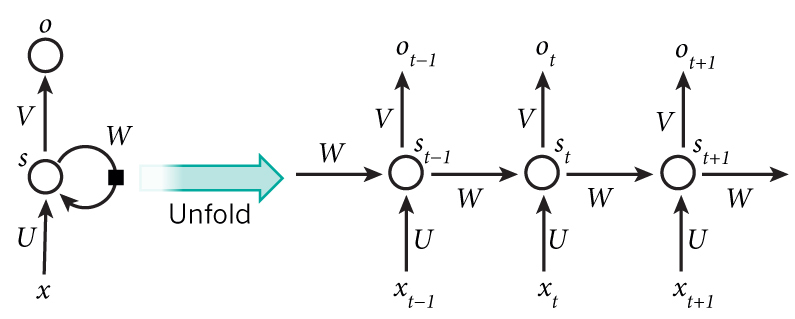
\includegraphics[width=0.8\linewidth]{images/RNN-unrolled.jpg} %source: http://www.wildml.com/2015/09/recurrent-neural-networks-tutorial-part-1-introduction-to-rnns/
\caption{A recurrent neural network in which each state (hidden unit) is passed to the next one. $x_t$ and $o_t$ are respectively the input and output at time step $t$. $s_t$ is the output of a hidden layer and depends on the input and the hidden unit at the previous time step: $s_t = U*x_t + W*s_{t-1}$. Note that the same weights $U$, $V$ and $W$ are used at each time step. Source: \cite{LeCun2015DeepLearning}.}
\label{fig:rnnunrolled}
\end{figure}
%The above diagram has outputs at each time step, but depending on the task this may not be necessary. For example, when predicting the sentiment of a sentence we may only care about the final output, not the sentiment after each word. Similarly, we may not need inputs at each time step. The main feature of an RNN is its hidden state, which captures some information about a sequence.

Training them was a problem because of the vanishing or exploding gradients, as these gradients either shrink or grow at every time step. Theoretical and empirical evidence has shown that it is hard for these kind of networks to store information long enough and that they have difficulties to learn the long-term dependencies \citep{bengio1994learning}.\\ %Sources for this: http://people.idsia.ch/~juergen/SeppHochreiter1991ThesisAdvisorSchmidhuber.pdf and http://www-dsi.ing.unifi.it/~paolo/ps/tnn-94-gradient.pdf

To learn RNNs, we also need to change the backpropagation algorithm in order to handle with the different time steps. Here, the error (for one training example) is just the sum of the errors at every time step: $e = \sum_t e_t$. The adapted backpropagation algorithm, called backpropagation through time (BPTT), also just sums up the gradient at every time step for every set of weights:  $\frac{\partial E}{\partial W} = \sum_t \frac{\partial E_t}{\partial W}$. For the weights $U$ and $V$ of Figure \ref{fig:rnnunrolled}, the gradients are computed just as in normal backpropagation. For $W$ however, we depend on the previous state, which cannot simple be treated as a constant, and must be replaced as well. Because of this, we get:
\begin{equation}
\frac{\partial E_t}{\partial W} = \sum_{k=0}^t \frac{\partial E_t}{\partial \hat{y}_t} \frac{\partial \hat{y}_t}{\partial s_t} \frac{\partial s_t}{\partial s_k} \frac{\partial s_k}{\partial W}
\end{equation}
We see that training can be hard when the sequences are long, because we need to propagate back through the first time step.\\

For the \textit{tanh} and \textit{sigmoid} function, the derivative is $0$ at both ends. This means that the gradients in other layers will also go towards zero and for small values in the matrix multiplications the gradient values are shrinking exponentially fast and become nearly zero after a few time steps. Because of this, steps far away won't contribute much to what you're currently computing, and as such the long-term dependencies are small. If the values of the partial derivatives are high however, we could get exploding gradients. These are however easier to detect and solve, because the value of the gradients will be too high to be presented by a variable in the programming language. The problem can also easily be solved by restricting the value in a certain range.\\ %source: http://www.jmlr.org/proceedings/papers/v28/pascanu13.pdf
The problem of vanishing gradients can be solved by a better initialization of the weights, by regularization and by another non-linear function, namely the already explained \textit{ReLU}.
For this function, the derivative is either 0 (when $z<0$) or 1 ($\frac{\partial z}{\partial z} = 1$).\\

A way of solving this is using a long short-term memory. This is a combination of different units and has an explicit memory. One of the units has a connection with itself and is used to accumulate or forget the stored information. It can be learned using another unit to know when to forget something and when to remember past information.\\
An LSTM architecture consists of different parts:
\begin{itemize}
\item An input gate $i$ that determines how much of the newly calculated state should be let through into the memory: $i = \sigma (x_tU^i + s_{t-1}W^i)$.
\item A forget gate $f$ that determines how much of the previous state you want to let through: $f = \sigma (x_tU^f + s_{t-1}W^f)$.
\item An output gate $o$ that determines how much of the internal hidden state you want to output to the next layer: $o = \sigma (x_tU^o + s_{t-1}W^o)$.
\item A candidate hidden state $g$ that is based on the input of the current time step and the state of the previous time step: $g = tanh(x_tU^g + s_{t-1}W^g)$.
\item An internal memory $c_t$ that is the sum of a fraction of the memory of the previous time step (determined by the forget gate) and a fraction of the candidate state (determined by the input gate): $c_t = c_{t-1} \circ f + g \circ i$.
\item Finally, the output hidden state $s_t$ is a fraction of the $tanh$ of the memory $c_t$, determined by the output gate: $s_t = tanh(c_t) \circ o$
\end{itemize}
Here, $U^i$ is for example one of the weight vectors for the input gate. The $\sigma$ function means the sigmoid function. $\circ$ refers to the dot product, i.e. $x \circ y = \sum_i^N x_i y_i$.\\
We can almost get the original RNN by setting the input and output gate weights to 1 and the forget gate weights to 0. The only difference is the $tanh$ function used to compute the output hidden state, which squashes the result more (along with the $tanh$ used to compute the candidate hidden state).\\
Another kind of recurrent unit is the Gated Recurrent Unit (GRU), which was introduced by \cite{Cho2014LearningTranslation}. It is simpler than LSTM but yields similar results. A GRU unit consists of the following parts:
\begin{itemize}
\item The update gate $z$ determines how much of the previous memory we want to keep, based on the input and the previous hidden state: $z = \sigma (x_tU^z + s_{t-1}W^z)$.
\item The reset gate $r$ says how much of the previous hidden state we want to combine with the current input, based on the previous hidden state and the input themselves: $z = \sigma (x_tU^r + s_{t-1}W^r)$.
\item Again a candidate hidden state $h$ that actually combines the previous hidden state and the input, using its own weights and the information from the reset gate: $h = tanh(x_tU^h + (s_{t-1} \circ r)W^h)$.
\item A new output hidden state based that combines all the previous information: $s_t = (1-z) \circ h + z \circ s_{t-1}$.
\end{itemize}
As we can see, the non-linearity function $tanh$ is only used once here. We also have no internal memory $c_t$ here. Instead, we use the update gate $z$ to combine the forget and input gate of the LSTM. The reset gate here is applied to the previous hidden state. As such, resetting in the LSTM architecture is done here using both the update gate and the reset gate. By always setting the reset gate to $1$ and the update gate to $0$ we get again the classic RNN architecture.\\

Other networks with memory include a Neural Turing Machine, in which a tape-like memory is used from which the network can read or write.\\
Another kind is a memory network, in which a normal network is augmented by a associative memory.\\

\subsection{Dropout}
Dropout is a way to prevent overfitting. It does so by randomly leaving out some visible or hidden units. As a result, all incoming and outgoing connections to these temporarily removed units are also removed and the algorithm can't rely on these connections. The simplest way of determining if a unit has to be removed is by removing it with a certain probability $p$, e.g. $p=0.5$. This value can also be determined by validation. As each unit can be present or not when using the network, for $n$ units there are $2^n$ possible networks. By learning each time using a possibly different network, we have a way of combining multiple models where each model is trained only a few times and most weights are shared between other models. Dropout is only used when training. In the testing phase, no units are removed. Here, however, we multiple the outgoing weights of each unit by there probability $p$.
This is done to make sure that the the \textit{expected} output for any hidden unit is the same as the actual output at test time.

In deep learning there are usually millions of these weights which can each be adjusted and can influence the output.

\subsection{Optimization techniques}
Optimization techniques are ways of changing weights of a neural network using gradients for those weights. Some of these techniques may be better at avoiding getting stuck in local minima and may be faster. Here we discuss a few of these techniques.

\subsubsection{RMSProp}
%By \cite{Tieleman2012LectureMagnitude.}.

In RMSProp, we only use the sign of the gradient to update the weights. This allows us the escape from plateaus more quickly. This is combined with a step size, used to control how much of the gradient to apply to the weight, that is adapted for each weight separately. For example, we can multiply the step-size of a certain weight by a factor greater than one if its last 2 gradients agreed on the sign, and multiply the step-size by a value less than 1 otherwise. This means that, when the gradients agree on the direction, we give them more influence. If the are not consistent and disagree in subsequent steps, we decrease the influence. We can also put a limit on the step-size as to not let it grow to excessively low or high amounts.\\
By just using this, we would however have a problem of weights growing too high in unwanted situations. For example, when a gradient is for 9 times a small positive amount (e.g. $0.1$) and once a large negative amount (e.g. $-0.9$), we don't want to change the weights a lot because they balance each other out. Using the current algorithm however, the step-size and so the weights would become too high because we only look at the signs and not the magnitude of the gradients.\\
Notice that, right know, we are dividing by the size of the gradient in order to just get $+1$ or $-1$ depending on the sign. It is however better to divide each weight by a moving average of the squared weight using the gradients of the past steps:
\begin{align}
MeanSquare(w, t) &= \gamma * MeanSquare(w, t-1) + (1 - \gamma) * f'(\theta_t)^2 \\
v_{t+1} &= \frac{\alpha}{\sqrt{MeanSquare(w,t)}}f'(\theta_t)
\end{align}
Where $f'(\theta_t)$ is the gradient, $\alpha$ is the learning rate and $v_{t+1}$ is the eventual update.

\section{DQN}
%Original paper by \cite{Mnih2015Human-levelLearning}.\\
A deep Q-network (DQN), presented in \cite{Mnih2015Human-levelLearning}, aims to combine deep learning with reinforcement learning. It applies a convolutional neural network to high-dimensional sensory inputs such as the pixels of a game screen in order to approximate an action-value function $Q^{*}(s,a)$. This is parametrised by the weights of the convolutional neural network, thus being $Q(s;a;\theta_i)$. Past experiences are also reused and the Q value function used to select action is only periodically updated to the most recently learned one in order to reduce instability.\\

This instability is caused by using a nonlinear function to approximate the action-value function and by the correlation between subsequent observations. Small changes in the $Q$ value can lead to big changes in the policy and because of that the data distribution and the correlations between the action-values $Q(s,a)$ and the target values $r+\gamma \max_{a'} Q(s',a')$ can also change a lot. The action that is selected determines which states that will be observed next.

Experience replay solves the problem of having correlated subsequent observations and changing data distributions by randomizing used mini-batches of the data on which is learned. In each iteration, these random mini-batches of saved experiences are used for applying Q-learning updates. Experiences can be used multiple times, which results in an efficient use of the available data.\\
For the replay memory, all the encountered experiences can be used or only the $N$ most recent ones. Here, however, it is possible that we forget experiences that may be important. Because we use uniform sampling to determine which experiences to use, we also give no extra importance (i.e. more probability) to more useful experiences.

A second improvement is to only update the used target function every $C$ steps. This helps to reduce the correlation between the action-value function values and the target values, as for example $Q(s_t, a_t)$ can have an influence on $Q(s_{t+1},a)$. To do this, we copy the current network weights to obtain an action-value function $\hat{Q}$ to generate target values $y_j$. By doing this, we add a delay between the time an update to $Q$ is made and the time the update affects the targets $y_j$, making divergence or oscillations much more unlikely.

The loss function used to update the weights of the parametrised action-value function is:
\begin{equation}
L_i(\theta_i) = E_{s,a,r,s'} \sim U(D) \big [ (r + \gamma \max_{a'} Q(s',a'; Q^{-}_i - Q(s,a;\theta_i)^2 \big ]
\end{equation}
Where $U(D)$ means that we take a uniformly random subset of the data set $D$. $\theta^{-}_i$ are the network parameters used to compute the target value. $\gamma$ determines the importance of future rewards. Instead of stochastic gradient descent, RMSProp is used here to update the weights.\\

The deep convolutional neural network gets as input the pixel colours of a game screen and has an output unit for every possible action. As such, we can compute the action-value function for every action when being in a certain state using only one forward pass.\\

To select an action, we can use the classic action selection policies such as $\epsilon$-greedy and softmax. Using these policies, we can learn off-policy because we don't always choose the action with the highest action-value. The value of respectively $\epsilon$ or $\tau$ in these mentioned policies can change over time to get closer to on-policy.\\

All rewards were clipped between -1 and 1 to limit the scale of derivatives and as such the amount of change of the weights. It also allows for using the same learning rate for multiple games.\\
\todo{Better explain gradient descent step?}
This results in the following pseudo-code:\\
\begin{algorithm}[H]
\DontPrintSemicolon
Initialize replay memory D to capacity N\;
Initialize action-value function $Q$ with random weights $\theta$\;
Initialize target action-value function $\hat{Q}$ with weights $\theta^- = \theta$\;
\For{episode = 1, M} {
	Initialize sequence $s_1 = \{x_1\}$ and preprocessed sequence $\phi_1 = \phi(s_1)$\;
    \For{$t=1,T$} {
    	With probability $\epsilon$ select a random action $a_t$\;
        otherwise select $a_t = \argmax_a Q(\phi(s_t),a;\theta)$\;
        Take action $a_t$ and observe reward $r_t$ and new image $x_{t+1}$\;
        $s_{t+1} \gets s_t,a_t,x_{t+1}$\;
        Preprocess $\phi_{t+1} \gets \phi(s_{t+1})$\;
        Store transition $(\phi_t,a_t,r_t,\phi_{t+1})$ in $D$\;
        Sample random minibatch of transitions $(\phi_j,a_j,r_j,\phi_{j+1})$ from $D$\;
        \eIf{episode terminates at step $j+1$} {
        	$y_j \gets r_j$\;
        }{
        	$y_j \gets r_j + \gamma \max_{a'} \hat{Q}(\phi_{j+1},a';\theta^-)$\;
        }
        Perform a gradient descent step on $(y_j - Q(\phi_j,a_j;\theta))^2$ with respect to the network parameters $\theta$\;
        Every $C$ steps reset $\hat{Q} \gets Q$\;
    }
}
\caption{Deep Q-learning with experience replay. Source: \cite{mnih2013playing}.}
\end{algorithm}

\subsection{Continuous control with deep reinforcement learning}
It is also possible to use an Actor-critic algorithm along with a replay buffer like in the DQN algorithm \citep{Mnih2015Human-levelLearning}. This idea is presented by \cite{Lillicrap2015ContinuousLearning}
%Uses Actor-critic with replay and (slightly) different target value function.

For the critic, a function approximator with the following loss is used:
\begin{equation}
L(\theta^Q) = E_{s_t \sim \rho^{\beta}, a_t \sim \beta, r_t \sim E} \big [ (Q(s_t, a_t \vert \theta^Q) - y_t)^2 \big ]
\end{equation}
Where
\begin{equation}
y_t = r(s_t,a_t) + \gamma Q(s_t, \mu(s_{t+1}) \vert \theta^Q)
\end{equation}
$\mu(s_t \vert \theta^Q)$ is a function that specifies the policy by mapping states to actions.
It can be seen that using the loss function we have a critic that is learned using the Bellman equation, just like in Q-learning.\\

Instead of just copying the weights to the target value network every $C$ steps, we gradually move the target value network values towards the learned network values: $\theta' \leftarrow \tau \theta + (1-\tau) \theta'$ with $\tau \ll 1$. This has the effect that target values can only change slowly. This stability slows learning but helps to avoid divergence.\\

Most of the games have different scales for their state values. Possible solutions are to change the hyperparameters for each game individually or to scale the states manually. However, it is also possible to use a more general solution called batch normalization. Here, we scale normalize each dimension across the samples in a minibatch in order to have unit mean and variance. This minimizes the covariance shift during training.
To have more exploration, noise is added to the actor policy. This noise is generated using the Ornstein-Uhlenbeck process.

\section{Asynchronous Methods for Deep Reinforcement Learning}
%By \cite{Mnih2016AsynchronousLearning}.
In \cite{Mnih2016AsynchronousLearning} experience replay isn't used because of memory and computation usage and because it is off-policy, which means that it learns from data generated by a policy that may already be outdated. Instead, we use multiple agents (that use well-known reinforcement algorithms) that run in parallel but each running on a separate instance of the same type of environment. These all run on a multi-core CPU (i.e. on only one computer). Each of the agents use the same parameters $\theta$, but by using certain exploration policies, they are able to each explore a possibly different part of the state space. It is possible to use a different exploration policy for each agent as to maximize the exploration of different states. Each agent also calculates a gradient w.r.t. the parameters $\theta$ depending on its experience. These gradients are accumulated and after a certain number of steps they are applied to the parameters $\theta$. Because they are global, this update has an effect on all agents. After an amount (possibly the same amount as for the gradient update) of steps, the target network parameters $\theta^{-}$ can also be updated using the current parameters $\theta$.\\
In $n$-step Q-learning and advantage actor-critic, a forward-view is used instead of the more commonly used backward view (which uses eligibility traces). Forward view was found to be easier when training neural networks with momentum-based methods and backpropagation through time. To do this, we first compute a certain number of steps (or until the episode is over). Then, the gradients are computed for each state-action pair encountered since the last update. Each n-step update uses the longest possible n-step return resulting in a one-step update for the last state, a two-step update for the second last state, and so on for a total of up to the previously determined number of maximum allowed steps. These accumulated gradients are then immediately applied to $\theta$. This results in the following pseudo-code:\\
\begin{algorithm}[H]
\DontPrintSemicolon
\emph{// Assume global shared parameter vectors $\theta$ and $\theta_v$ and global shared counter $T=0$}\;
\emph{// Assume thread-specific parameter vectors $\theta'$ and $\theta'_v$}\;
Initialize thread step counter $t\gets 1$\;
\Repeat{$T > T_{max}$}{
	Reset gradients: $d\theta \gets 0$ and $d\theta_v \gets 0$\;
    Synchronize agent-specific parameters  $\theta'=\theta$ and $\theta'_v=\theta_v$\;
    $t_{start} \gets t$\;
    Initialize state $s_t$\;
    \Repeat{terminal $s_t$ \textbf{or} $t-t_{start}==t_{max}$}{
    	Perform $a_t$ according to policy $\pi (a_t|s_t;\theta')$\;
		Receive reward $r_t$ and new state $s_{t+1}$\;
        $t \gets t + 1$\;
        $T \gets T + 1$\;
        }
        $R =
    \left\{
    \begin{array}{l l}
      0  \quad & \text{if $s_t$ is terminal}\\
        V(s_t,\theta'_v) \quad & \text{otherwise // Bootstrap from last state}
    \end{array}\right.$
    \For {$i \in \{t-1,\ldots,t_{start} \}$} {
    	Accumulate gradients w.r.t. $\theta'$: $d\theta \gets d\theta + \nabla_{\theta'} \log\pi(a_i|s_i;\theta') (R - V(s_i;\theta'_v))$\;
        Accumulate gradients w.r.t. $\theta'_v$: $d\theta_v \gets d\theta_v + {\partial\left(R - V(s_i;\theta'_v)\right)^2}/{\partial \theta'_v}$\;
    }
    Perform asynchronous update of $\theta$ using $d\theta$ and of $\theta_v$ using $d\theta_v$\;
}
\caption{Asynchronous Advantage Actor Critic (A3C). Source: \cite{Mnih2016AsynchronousLearning}.}
\end{algorithm}

\section{Transfer learning}
%\cite{Taylor2009TransferSurvey}.
\todo{Say somewhere that a task is simply an Markov Decision Process}
Transfer learning involves the use of experience gained when learning one task to improve the performance on a different but related task. Here, we discuss a framework for transfer methods that can be used for reinforcement learning, closely following \cite{Taylor2009TransferSurvey}.\\

The transfer of knowledge always happens between one or more source tasks. First, an appropriate set of tasks must be selected. Afterwards, the transfer learning algorithm must learn how these source tasks are related to the target task.\\

To be able to transfer knowledge, some assumptions must be made about differences between the source tasks and the target task. This can be for example in the underlying dynamics of the environment, which can make the task harder or easier to solve, or different sets of possible actions at certain states. These differences define between which type of source and target tasks knowledge can be transferred. The differences between the source task(s) and target task can also make the knowledge transfer easier or harder, requiring the appropriate guidance by a human or a method that can overcome these differences in case of a fully autonomous transfer learner.\\
Multi-task learning is a special kind of task learning where the problems for the source and target tasks are drawn from the same distribution instead of having arbitrary source and target tasks. More specifically, the transition function is drawn from a fixed distribution of functions. For the mountain car environment , this may mean for example that the motor of the car differs in power in different tasks.\\

As was stated, first the set of source tasks needs to be selected. Again, this can be done by a human in case of a human-guided scenario. However, the selection may also be done by the agent itself. It can learn multiple source task and then use them all for transfer. Another possibility is to select the source tasks that are the most relevant and lead to highest performance for the target task. The agent may also just aim to avoid negative transfer, which means that the specific selection of source tasks leads to worse learning performance for the target task.
The agent could also modify the source task such that the knowledge transfer is the most useful in the target task.\\

Instead of just knowing that tasks are related, many methods also need to know how tasks are related, using task mappings. This is necessary to make the knowledge gained on the source tasks useful for the target task. Tasks may differ in state and action variables and the in the semantic meaning of them. In the mountain car environment, one can have a task where the goal is on the opposite side. As such, taking the action \texttt{Left} has a different meaning for these tasks. Actions in the two tasks must be mapped such that their effects are similar.\\
Again, these mappings can be provided by a human or they can be learned by the agent. Note that these mappings may be partial and not every action in the source task is mapped to an action in the target task or vice-versa. For states, it is also possible to map the states themselves instead of the state variables.\\
In multi-task learning, states and variables are the same and have the same meaning. Because of this, no task mapping is necessary in multi-task learning.\\

Task learning methods can also differ in the type of knowledge that is transferred between source and target tasks. This knowledge can be for example an action-value function, transitions or policy gradient parameters. For tasks that are closely related, detailed knowledge may be useful. Otherwise, high-level information may result in a better learning performance. The type of knowledge that is tranferred can also depend on the type of source and target tasks and on the task mappings.\\

Last, the task learning method may also restrict which reinforcement learning algorithms that can be used. It is possible for example that only a class of reinforcement learning algorithms or only one specific reinforcement learning algorithm can be used with the task learning method or that the algorithm is the same for both the source and target tasks. Ideally, the reinforcement learning algorithms can be chosen freely and may be selected based on the characteristics of the task.\\

\subsection{Metrics}
Several metrics exist to evaluate the learning performance and solution quality of transfer learning algorithms. Generally, one metric does not give a complete representation of the overall performance of the algorithm. Because of this, often multiple metrics are used.\\
Here we will list the most popular ones:
\begin{itemize}
    \item \textit{Jumpstart}: This is the initial improvement that the target task has over an algorithm that doesn't use knowledge transfer. However, no learning has occurred yet. Because of this, learning performance can't be measured. The metric also does not give an indication about the final performance, i.e. the performance after having learned.
    \item \textit{Asymptotic performance}: This is the opposite of \textit{jumpstart} performance and measures the performance improvement after having learned the target task. However, this is hard to measure because one has to know when the task learning algorithm converged. Furthermore, the task learning algorithm and the algorithm that doesn't use knowledge transfer may require a different training time in order to converge.
    \item \textit{Total reward}: This is the total reward that the algorithm has accumulated during learning, i.e. the area under the learning curve. In case of improvement, this area is bigger than when transfer learning isn't used. This can be achieved when the transfer learning algorithm has a higher learning rate. However, convergence is again an issue here. An algorithm that learns slower and thus takes more time to converge may accumulate a higher total reward than a faster algorithm that may even reach a higher performance. This metric is only useful for task that always have the same duration.
    \item \textit{Transfer ratio}: This is the ratio of the total reward improvement that the transfer learning algorithm has over the other algorithm. Because it uses the \textit{total reward} metric, it suffers from the same issues. Furthermore, it is also influenced by the reward structure. For example, an agent always receiving a reward of $+1$ at the end of the episode may result in a different ratio.
    \item \textit{Time to threshold}: This measures the time needed to reach a pre-defined performance. A transfer leraning may need less time to reach this threshold. The threshold needs to be defined manually and depends on the task domain and learning method.
\end{itemize}
A graph with 3 of the 5 metrics is shown in Figure~\ref{fig:TLmetrics}.
\begin{figure}[H]
    \centering
    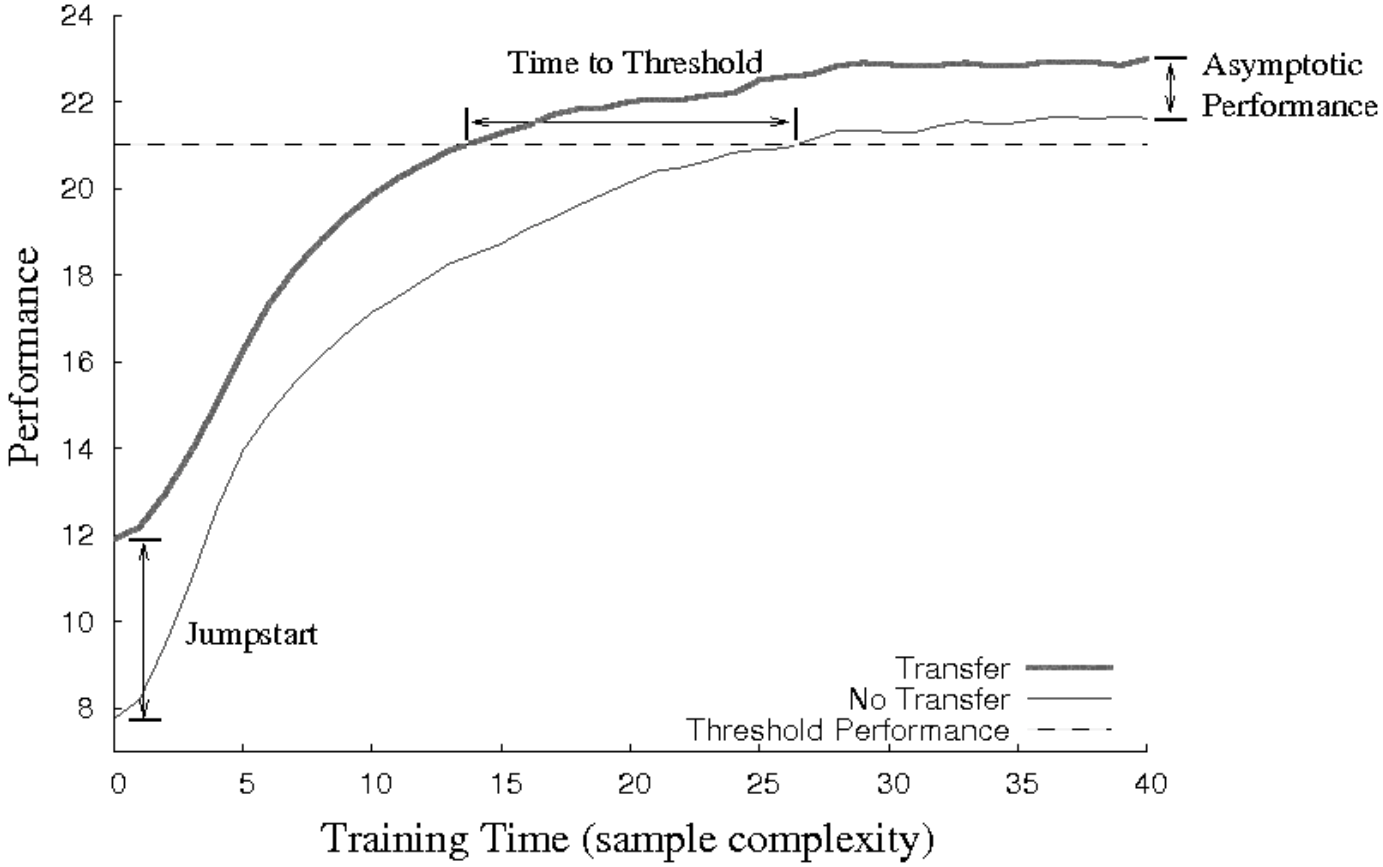
\includegraphics[width=\linewidth]{images/tlmetrics.png}
    \caption{A graph comparing the \textit{jumpstart}, \textit{time to threshold} and \textit{asymptotic performance} metrics between the algorithm that uses knowledge transfer and the one that doesn't. Note that here the transfer learning algorithm performs better on all three metrics. It can also be seen that the total reward is higher. Source: \cite{Taylor2009TransferSurvey}.}
    \label{fig:TLmetrics}
\end{figure}
Instead of comparing the transfer learning algorithm with a algorithm that doesn't use knowledge transfer, it is also possible to compare the algorithm with the performance of humans (by averaging their performances). However, metrics must be chosen carefully such that they don't favor the algorithm or the human and they can be abused.

\subsection{Using Task Features for Zero-Shot Knowledge Transfer in Lifelong Learning}
An extra problem is to learn multiple variations of environment instead of just one. This means that for each of these tasks the transition function is slightly different, while keeping the same action space and state space.
In \cite{Isele2016UsingLearning}, a method is presented that learns these task simultaneously by using a predefined description for each task. When a new task arrives along with its features, obtained from its task descriptor, a policy can be generated that immediately results in a good performance, even though the algorithm was not applied on that task before and the task descriptor, task order and task distribution was not known on beforehand. This way, knowledge transfer can take place without the need of training data to identify relationships across tasks. For each subsequent task, the policy and feature vector are iteratively improved.\\
%factorization: ontbinding in factoren: bijv. 15=3*5
First, it is assumed that the policy parameters for every task $t$ can be factorized using a shared knowledge base $L \in \mathbb{R}^{d \times k}$: $\theta^{(t)} = Ls^{(t)}$. $s^{(t)} \in \mathbb{R}^{(k)}$ are the sparse coefficients over the basis, i.e. the latent representation of the policy's parameters for task $t$. $L$ is able to capture relationships among policies as this is used to compute every policy, whereas there is a sparse representation for computed for each task separately.\\
The features of the task are obtained by (possibly non-linear) feature extractors applied on the descriptor of the task: $\phi(m^{(t)}) \in \mathbb{R}^{d_m}$. These features can also be linearly factorized using another shared knowledge base $D \in \mathbb{R}^{d_m \times k}$: $\phi(m^{(t)}) = Ds^{(t)}$, where the same sparse representation is used as the one used to compute the policy. Both knowledge bases provide information about the task and because of this they share the same coefficient vectors $S$. We then used coupled dictionary optimization techniques from the sparse coding literature to optimize these dictionaries. They are updated iteratively based on trajectories samples from the current task.\\
When a new task arrives, with its task descriptor, we search for the coefficients $s^{(t_{new})}$ that minimize the difference between the extracted features and the reconstruction of it using the shared knowledge base $D$. Using these coefficients, we can compute the policy parameters using $\theta = Ls^{(t_{new})}$. Afterwards, we can iterate again to improve $s$ and the knowledge bases.

\section{Related work}
% Types of knowledge that is transferred: Value functions, features extracted from value functions, heuristics, policies
% Different representation types: Graphs, relational representation, tables

% Representation transfer
    % options

% separation in subtasks

% Relational RL

% transferring instances
% transferring advice/preferences
Transfer learning methods for reinforcement learning can first be divided into 2 groups: methods that use task mappings and methods that don't. Will will first discuss methods that don't use task mappings. Afterwards we will only briefly discuss methods that use task mappings, as these are less related to our proposed method.

\subsection{Methods that don't use task mappings} % (fold)
\label{sub:methods_that_don_t_use_task_mappings}
%Also put this in one of the subdivisions below or not?
In of the earliest works of transfer learning used for reinforcement learning \citep{conf/ijcai/SelfridgeSB85}, the transition function was gradually changed as to make the task harder. A cart pole task was used where the pole was long and light at first, but was made shorter and heavier over time. The total time spent learning on the sequence of gradually modified tasks was shorter than when trying to solve the hardest task directly.\\

Earlier work was generally focused on transferring from one source task to a target task, while in recent research, most of the times a more general scenario with possibly multiple sources is considered.
%Say something about further grouping of methods

%Here something about source-to-task
\subsubsection{Single source} % (fold)
\label{ssub:single_source}

% subsubsection single_source (end)

%Here something about sources-to-task
\subsubsection{Multiple sources} % (fold)
\label{ssub:multiple_sources}
One approach, presented in , is to transfer transitions (also called \textit{instances} or \textit{samples}) gather from the source tasks to the target task.
% subsubsection multiple_sources (end)

% subsection methods_that_don_t_use_task_mappings (end)

\subsection{Methods that use task mappings} % (fold)
\label{sub:methods_that_use_task_mappings}

% subsection methods_that_use_task_mappings (end)

\section{Proposed algorithm}
\label{sec:proposed_algorithm} % (fold)
Our approach only uses a latent basis over the policy space instead of using one over the policy space and another one over the descriptor space like is done by \cite{Isele2016UsingLearning}. Again, for a task $(t)$, we can reconstruct the policy using the shared basis $L$ and the sparse coefficients over this basis for that specific task $s^{(t)}$: $\theta^{(t)} = Ls^{(t)}$, with $\theta^{(t)} \in \mathbb{R}^d$, $L \in \mathbb{R}^{d \times k}$ and $s^{(t)} \in \mathbb{R}^k$.\\

The first set of tasks can be learned in two ways. One can either learn these tasks sequentially or asynchronous. In the sequential way, we collect trajectories and calculate the gradients for every task after another. This is calculated for every episode of a task like in the \texttt{REINFORCE} algorithm, i.e. with likelihood ratios using discounted rewards as a sample for the $Q$ values of the policy.\\
Once this is done, we sum and apply the gradients of every task. The learning process for this set of tasks then stops when a certain number of updates have been applied.\\
In the asynchronous way, learning is executed in parallel and for each task, a number of updates are executed on its own. Trajectories are collected for each task continuously and its gradients are applied immediately after they are calculated. This means that they are not first summed as in the sequential method.\\
Afterwards, we learn the new task separately for a certain number of updates.\\
\todo{Use ref instead}
This results in the following pseudo code for the source tasks:\\
\begin{algorithm}[H]
\DontPrintSemicolon
\emph{// Assume global shared parameter vector $\theta_g$ and global shared counter $T \gets 0$}\;
\emph{// Assume thread-specific parameter vector $\theta_g'$}\;
Initialize thread-specific paramter vector $\theta^{(t)}$\;
Initialize thread step counter $t\gets 1$\;
\Repeat{$T > T_{max}$}{
    Reset gradients: $d\theta_g \gets 0$\;
    Synchronize agent-specific parameters  $\theta_g' \gets \theta_g$\;
    $t_{start} \gets t$\;
    Initialize state $s_t$\;
    \Repeat{terminal $s_t$ \textbf{or} $t-t_{start} == t_{max}$}{
        Perform $a_t$ according to policy $\pi(a_t|s_t;\theta' \cup \theta^{(t)})$\;
        Receive reward $r_t$ and new state $s_{t+1}$\;
        $t \gets t + 1$\;
        $T \gets T + 1$\;
        }
    \For {$i \in \{t-1,\dots,t_{start} \}$} {
        %Accumulate gradients w.r.t. $\theta'$: $d\theta \gets d\theta + \nabla_{\theta'} \log\pi(a_i|s_i;\theta') (R - V(s_i;\theta'_v))$\;
        Accumulate gradients w.r.t. $\theta' \cup \theta^{(t)}$: $\theta \gets \theta + \alpha \nabla_{\theta \cup \theta^{(t)}} \log \pi_{\theta \cup \theta^{(t)}}(s_t,a_t)v_t$\;
    }
    Perform asynchronous update of $\theta$ using $d\theta$ and of $\theta_v$ using $d\theta_v$\;
}
\caption{Asynchronous knowledge transfer agent for source task}
\end{algorithm}
For the target task, the pseudo code is the following:\\
\begin{algorithm}[H]
\DontPrintSemicolon
\emph{// Assume global shared parameter vector $\theta_g$ and global shared counter $T \gets 0$}\;
\emph{// Assume thread-specific parameter vector $\theta_g'$}\;
Initialize thread-specific paramter vector $\theta^{(t)}$\;
Initialize thread step counter $t\gets 1$\;
\Repeat{$T > T_{max}$}{
    $t_{start} \gets t$\;
    Initialize state $s_t$\;
    \Repeat{terminal $s_t$ \textbf{or} $t-t_{start} == t_{max}$}{
        Perform $a_t$ according to policy $\pi(a_t|s_t;\theta_g \cup \theta^{(t)})$\;
        Receive reward $r_t$ and new state $s_{t+1}$\;
        $t \gets t + 1$\;
        $T \gets T + 1$\;
        }
    \For {$i \in \{t-1,\dots,t_{start} \}$} {
        %Accumulate gradients w.r.t. $\theta'$: $d\theta \gets d\theta + \nabla_{\theta'} \log\pi(a_i|s_i;\theta') (R - V(s_i;\theta'_v))$\;
        Accumulate gradients w.r.t. $\theta^{(t)}$: $\theta \gets \theta^{(t)} + \alpha \nabla_{\theta^{(t)}} \log \pi_{\theta^{(t)}}(s_t,a_t)v_t$\;
    }
    Perform asynchronous update of $\theta$ using $d\theta$ and of $\theta_v$ using $d\theta_v$\;
}
\caption{Knowledge transfer agent for target task}
\end{algorithm}
% section proposed_algorithm (end)

\section{Experimental setup}
Experiments were executed on variations of the cart-pole environment.
In this 2-dimensional environment, a pole is placed vertically on a cart. The goal in this environment is to keep the pole balanced vertically (i.e. keep the angle of the pole between thresholds) and to keep the cart between 2 borders. The state is defined by 4 continuous-valued attributes: the position of the cart, the velocity of the cart, the angle of the pole and the angular velocity of the pole. A discrete value of $1$ is given as a reward each time the pole is balanced and the cart is between bounds. If this isn't the case, the episode ends. An agent can either move left or right. It can't stay at its current position. For the experiments, an implementation by \cite{Brockman2016OpenAIGym} was used.\\

In the experiment, first a number of environments are randomly generated. The environment for each task can differ for a predefined number of attributes, of which the values can each be in a certain range. For a cart-pole task, this can be the length and the mass of the pole.\\
Then a number of tasks were learned that can update both the shared knowledge base and their own sparse representation. After a number of epochs, i.e. updates to these variables, we stop with learning these tasks. Instead, we learn to solve a new task for which we hadn't learned its sparse representation. Here however, only the sparse representation can be updated and not the shared knowledge base.\\
This learning process is repeated 20 times with the same set of environments. However it is possible that the attributes of each environment may be similar and thus knowledge transfer may be trivial. Because of this, we generate 10 times a new set of environments and execute 20 runs with them as explained before.\\
Afterwards the rewards are averaged over all the runs and results of different environment sets.\\
Trajectories for both sets of tasks contained of maximally 200 steps. This could be less in case the environment was in an end state. In case of the cart-pole environment, this can mean for example that the cart tried to cross the left or right border or that the pole fell down.\\
Hyperparameters, such as the learning rate of neural networks, were chosen by iteratively executing the previously mentioned experiment. Possible values for each hyperparameter were chosen manually.

\begin{figure}[H]
    \centering
    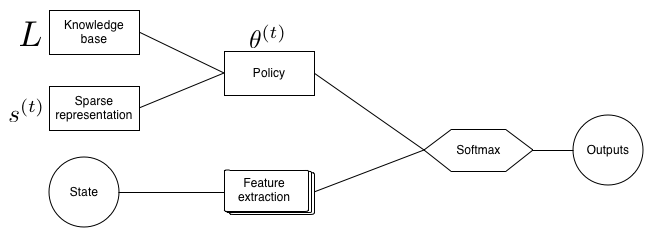
\includegraphics[width=\linewidth]{images/knowledge_transfer.png}
    \caption{Artificial neural network architecture.}
    \label{fig:algonn}
\end{figure}
\section{Results}
\section{Conclusion}
\subsubsection*{Acknowledgments}

\bibliographystyle{apalike}
\bibliography{Mendeley.bib}
\end{document}